\documentclass[12pt,a4paper,oneside]{book}
%% -----
%% memoir
%% -----
\usepackage{enumerate}
\usepackage[shortlabels]{enumitem}
\usepackage{multirow}
\usepackage{makecell}
\usepackage{booktabs}
\usepackage{longtable}
\usepackage{caption}

% --------------------------
\usepackage{amssymb, amsmath, amsbsy} % simbolitos
\usepackage{upgreek} % para poner letras griegas sin cursiva
\usepackage{mathdots} % para el comando \iddots
\usepackage{mathrsfs} % para formato de letra
\usepackage{stackrel} % para el comando \stackbin

\usepackage{rotating}
\usepackage{glossaries}

\usepackage[T1]{fontenc}
\usepackage{charter}

\usepackage{setspace}

\usepackage{vmargin}


%
% Definimos  el   comando  \compilaCapitulo,  que   luego  se  utiliza
% (opcionalmente) en config.tex. QuedarXa  mejor si tambiXn se definiera
% en  ese fichero,  pero por  el modo  en el  que funciona  eso  no es
% posible. Puedes consultar la documentaciXn de ese fichero para tener
% mXs  informaciXn. Definimos tambiXn  \compilaApendice, que  tiene el
% mismo  cometido, pero  que se  utiliza para  compilar  Xnicamente un
% apXndice.
%
%
% Si  queremos   compilar  solo   una  parte  del   documento  podemos
% especificar mediante  \includeonly{...} quX ficheros  son los Xnicos
% que queremos  que se incluyan.  Esto  es Xtil por  ejemplo para sXlo
% compilar un capXtulo.
%
% El problema es que todos aquellos  ficheros que NO estXn en la lista
% NO   se  incluirXn...  y   eso  tambiXn   afecta  a   ficheros  de
% la plantilla...
%
% Total,  que definimos  una constante  con los  ficheros  que siempre
% vamos a querer compilar  (aquellos relacionados con configuraciXn) y
% luego definimos \compilaCapitulo.
\newcommand{\ficherosBasicosTeXiS}{%
TeXiS/TeXiS_pream,TeXiS/TeXiS_cab,TeXiS/TeXiS_bib,TeXiS/TeXiS_cover,%
TeXiS/TeXiS_part%
}
\newcommand{\ficherosBasicosTexto}{%
constantes,guionado,Cascaras/bibliografia,config%
}
\newcommand{\compilaCapitulo}[1]{%
\includeonly{\ficherosBasicosTeXiS,\ficherosBasicosTexto,Capitulos/#1}%
}

\newcommand{\compilaApendice}[1]{%
\includeonly{\ficherosBasicosTeXiS,\ficherosBasicosTexto,Apendices/#1}%
}

%- - - - - - - - - - - - - - - - - - - - - - - - - - - - - - - - - - -
%            PreXmbulo del documento. Configuraciones varias
%- - - - - - - - - - - - - - - - - - - - - - - - - - - - - - - - - - -

% Define  el  tipo  de  compilaciXn que  estamos  haciendo.   Contiene
% definiciones  de  constantes que  cambian  el  comportamiento de  la
% compilaciXn. Debe incluirse antes del paquete TeXiS/TeXiS.sty
%---------------------------------------------------------------------
%
%                          config.tex
%
%---------------------------------------------------------------------
%
% Contiene la  definici�n de constantes  que determinan el modo  en el
% que se compilar� el documento.
%
%---------------------------------------------------------------------
%
% En concreto, podemos  indicar si queremos "modo release",  en el que
% no  aparecer�n  los  comentarios  (creados  mediante  \com{Texto}  o
% \comp{Texto}) ni los "por  hacer" (creados mediante \todo{Texto}), y
% s� aparecer�n los �ndices. El modo "debug" (o mejor dicho en modo no
% "release" muestra los �ndices  (construirlos lleva tiempo y son poco
% �tiles  salvo  para   la  versi�n  final),  pero  s�   el  resto  de
% anotaciones.
%
% Si se compila con LaTeX (no  con pdflatex) en modo Debug, tambi�n se
% muestran en una esquina de cada p�gina las entradas (en el �ndice de
% palabras) que referencian  a dicha p�gina (consulta TeXiS_pream.tex,
% en la parte referente a show).
%
% El soporte para  el �ndice de palabras en  TeXiS es embrionario, por
% lo  que no  asumas que  esto funcionar�  correctamente.  Consulta la
% documentaci�n al respecto en TeXiS_pream.tex.
%
%
% Tambi�n  aqu� configuramos  si queremos  o  no que  se incluyan  los
% acr�nimos  en el  documento final  en la  versi�n release.  Para eso
% define (o no) la constante \acronimosEnRelease.
%
% Utilizando \compilaCapitulo{nombre}  podemos tambi�n especificar qu�
% cap�tulo(s) queremos que se compilen. Si no se pone nada, se compila
% el documento  completo.  Si se pone, por  ejemplo, 01Introduccion se
% compilar� �nicamente el fichero Capitulos/01Introduccion.tex
%
% Para compilar varios  cap�tulos, se separan sus nombres  con comas y
% no se ponen espacios de separaci�n.
%
% En realidad  la macro \compilaCapitulo  est� definida en  el fichero
% principal tesis.tex.
%
%---------------------------------------------------------------------


% Comentar la l�nea si no se compila en modo release.
% TeXiS har� el resto.
% ���Si cambias esto, haz un make clean antes de recompilar!!!
\def\release{1}


% Descomentar la linea si se quieren incluir los
% acr�nimos en modo release (en modo debug
% no se incluir�n nunca).
% ���Si cambias esto, haz un make clean antes de recompilar!!!
%\def\acronimosEnRelease{1}


% Descomentar la l�nea para establecer el cap�tulo que queremos
% compilar

% \compilaCapitulo{01Introduccion}
% \compilaCapitulo{02EstructuraYGeneracion}
% \compilaCapitulo{03Edicion}
% \compilaCapitulo{04Imagenes}
% \compilaCapitulo{05Bibliografia}
% \compilaCapitulo{06Makefile}

% \compilaApendice{01AsiSeHizo}

% Variable local para emacs, para  que encuentre el fichero maestro de
% compilaci�n y funcionen mejor algunas teclas r�pidas de AucTeX
%%%
%%% Local Variables:
%%% mode: latex
%%% TeX-master: "./Tesis.tex"
%%% End:


% Paquete de la plantilla
\usepackage{TeXiS/TeXiS}

% Incluimos el fichero con comandos de constantes
\def\titulo{\textsc Uso de herramientas de la computaci\'on en la
nube y su efecto en la gesti\'on de las MiPYME pertenecientes al Programa del
Centro de Desarrollo Empresarial del Cusco, 2017}

\def\autor{Alex Irmel Oviedo Solis}


% Sacamos en el log de la compilaciXn el copyright
\typeout{Copyright Alex Irmel Oviedo Solis}

%
% "Metadatos" para el PDF
%
\ifpdf\hypersetup{%
    pdftitle = {\titulo},
    pdfsubject = {Tesis de maestría},
    pdfkeywords = {MiPYME,Cloud Computing, tesis, trabajo de
      investigación, trabajo de Master},
    pdfauthor = {\textcopyright\ \autor},
    pdfcreator = {\LaTeX\ con el paquete \flqq hyperref\frqq},
    pdfproducer = {pdfeTeX-0.\the\pdftexversion\pdftexrevision},
    }
    \pdfinfo{/CreationDate (\today)}
\fi


%- - - - - - - - - - - - - - - - - - - - - - - - - - - - - - - - - - -
%                        Documento
%- - - - - - - - - - - - - - - - - - - - - - - - - - - - - - - - - - -
\begin{document}

\fontfamily{bch}
\selectfont
% Incluimos el  fichero de definiciXn de guionado  de algunas palabras
% que LaTeX no ha dividido como deberXa
%----------------------------------------------------------------
%
%                          guionado.tex
%
%----------------------------------------------------------------
%
% Fichero con algunas divisiones de palabras que LaTeX no
% hace correctamente si no se le da alguna ayuda.
%
%----------------------------------------------------------------

\hyphenation{
% a
abs-trac-to
abs-trac-tos
abs-trac-ta
abs-trac-tas
ac-tua-do-res
a-gra-de-ci-mien-tos
ana-li-za-dor
an-te-rio-res
an-te-rior-men-te
apa-rien-cia
a-pro-pia-do
a-pro-pia-dos
a-pro-pia-da
a-pro-pia-das
a-pro-ve-cha-mien-to
a-que-llo
a-que-llos
a-que-lla
a-que-llas
a-sig-na-tu-ra
a-sig-na-tu-ras
a-so-cia-da
a-so-cia-das
a-so-cia-do
a-so-cia-dos
au-to-ma-ti-za-do
ad-mi-nis-tra-ci\'on
ad-mi-nis-tra-ti-vas
% b
batch
bi-blio-gra-f\'ia
bi-blio-gr\'a-fi-cas
bien
bo-rra-dor
boo-l-ean-expr
% c
ca-be-ce-ra
call-me-thod-ins-truc-tion
cas-te-lla-no
cir-cuns-tan-cia
cir-cuns-tan-cias
co-he-ren-te
co-he-ren-tes
co-he-ren-cia
co-li-bri
co-men-ta-rio
co-mer-cia-les
co-no-ci-mien-to
cons-cien-te
con-si-de-ra-ba
con-si-de-ra-mos
con-si-de-rar-se
cons-tan-te
cons-trucci\'on
cons-tru-ye
cons-tru-ir-se
con-tro-le
co-rrec-ta-men-te
co-rres-pon-den
co-rres-pon-dien-te
co-rres-pon-dien-tes
co-ti-dia-na
co-ti-dia-no
crean
cris-ta-li-zan
cu-rri-cu-la
cu-rri-cu-lum
cu-rri-cu-lar
cu-rri-cu-la-res
% d
de-di-ca-do
de-di-ca-dos
de-di-ca-da
de-di-ca-das
de-rro-te-ro
de-rro-te-ros
de-sa-rro-llo
de-sa-rro-llos
de-sa-rro-lla-do
de-sa-rro-lla-dos
de-sa-rro-lla-da
de-sa-rro-lla-das
de-sa-rro-lla-dor
de-sa-rro-llar
des-cri-bi-re-mos
des-crip-ci\'on
des-crip-cio-nes
des-cri-to
des-pu\'es
de-ta-lla-do
de-ta-lla-dos
de-ta-lla-da
de-ta-lla-das
di-a-gra-ma
di-a-gra-mas
di-se-\~nos
dis-po-ner
dis-po-ni-bi-li-dad
do-cu-men-ta-da
do-cu-men-to
do-cu-men-tos
% e
edi-ta-do
e-du-ca-ti-vo
e-du-ca-ti-vos
e-du-ca-ti-va
e-du-ca-ti-vas
e-la-bo-ra-do
e-la-bo-ra-dos
e-la-bo-ra-da
e-la-bo-ra-das
es-co-llo
es-co-llos
es-tu-dia-do
es-tu-dia-dos
es-tu-dia-da
es-tu-dia-das
es-tu-dian-te
e-va-lua-cio-nes
e-va-lua-do-res
exis-ten-tes
exhaus-ti-va
ex-pe-rien-cia
ex-pe-rien-cias
% f
for-ma-li-za-do
% g
ge-ne-ra-ci\'on
ge-ne-ra-dor
ge-ne-ra-do-res
ge-ne-ran
% h
he-rra-mien-ta
he-rra-mien-tas
% i
i-dio-ma
i-dio-mas
im-pres-cin-di-ble
im-pres-cin-di-bles
in-de-xa-do
in-de-xa-dos
in-de-xa-da
in-de-xa-das
in-di-vi-dual
in-fe-ren-cia
in-fe-ren-cias
in-for-ma-ti-ca
in-gre-dien-te
in-gre-dien-tes
in-me-dia-ta-men-te
ins-ta-la-do
ins-tan-cias
% j
% k
% l
len-gua-je
li-be-ra-to-rio
li-be-ra-to-rios
li-be-ra-to-ria
li-be-ra-to-rias
li-mi-ta-do
li-te-ra-rio
li-te-ra-rios
li-te-ra-ria
li-te-ra-rias
lo-tes
% m
ma-ne-ra
ma-nual
mas-que-ra-de
ma-yor
me-mo-ria
mi-nis-te-rio
mi-nis-te-rios
mo-de-lo
mo-de-los
mo-de-la-do
mo-du-la-ri-dad
mo-vi-mien-to
% n
na-tu-ral
ni-vel
nues-tro
% o
obs-tan-te
o-rien-ta-do
o-rien-ta-dos
o-rien-ta-da
o-rien-ta-das
% p
pa-ra-le-lo
pa-ra-le-la
par-ti-cu-lar
par-ti-cu-lar-men-te
pe-da-g\'o-gi-ca
pe-da-g\'o-gi-cas
pe-da-g\'o-gi-co
pe-da-g\'o-gi-cos
pe-rio-di-ci-dad
per-so-na-je
plan-te-a-mien-to
plan-te-a-mien-tos
po-si-ci\'on
pre-fe-ren-cia
pre-fe-ren-cias
pres-cin-di-ble
pres-cin-di-bles
pri-me-ra
pro-ble-ma
pro-ble-mas
pr\'o-xi-mo
pu-bli-ca-cio-nes
pu-bli-ca-do
% q
% r
r\'a-pi-da
r\'a-pi-do
ra-zo-na-mien-to
ra-zo-na-mien-tos
re-a-li-zan-do
re-fe-ren-cia
re-fe-ren-cias
re-fe-ren-cia-da
re-fe-ren-cian
re-le-van-tes
re-pre-sen-ta-do
re-pre-sen-ta-dos
re-pre-sen-ta-da
re-pre-sen-ta-das
re-pre-sen-tar-lo
re-qui-si-to
re-qui-si-tos
res-pon-der
res-pon-sa-ble
% s
se-pa-ra-do
si-guien-do
si-guien-te
si-guien-tes
si-guie-ron
si-mi-lar
si-mi-la-res
si-tua-ci\'on
% t
tem-pe-ra-ments
te-ner
trans-fe-ren-cia
trans-fe-ren-cias
% u
u-sua-rio
Unreal-Ed
% v
va-lor
va-lo-res
va-rian-te
ver-da-de-ro
ver-da-de-ros
ver-da-de-ra
ver-da-de-ras
ver-da-de-ra-men-te
ve-ri-fi-ca
% w
% x
% y
% z
}
% Variable local para emacs, para que encuentre el fichero
% maestro de compilaci�n
%%%
%%% Local Variables:
%%% mode: latex
%%% TeX-master: "./Tesis.tex"
%%% End:


% Marcamos  el inicio  del  documento para  la  numeraciXn de  pXginas
% (usando nXmeros romanos para esta primera fase).
\frontmatter

%---------------------------------------------------------------------
%
% Fichero que contiene la configuraci�n de la portada y de la
% primera hoja del documento.
%
%---------------------------------------------------------------------
\institucion{%
UNIVERSIDAD ANDINA DEL CUSCO\\[0.2em]
ESCUELA DE POSGRADO\\[0.2em]
MAESTRIA EN ADMINISTRACI'ON DE NEGOCIOS
}

% Pueden configurarse todos los elementos del contenido de la portada
% utilizando comandos.

%%%%%%%%%%%%%%%%%%%%%%%%%%%%%%%%%%%%%%%%%%%%%%%%%%%%%%%%%%%%%%%%%%%%%%
% T�tulo del documento:
% \tituloPortada{titulo}
% Nota:
% Si no se define se utiliza el del \titulo. Este comando permite
% cambiar el t�tulo de forma que se especifiquen d�nde se quieren
% los retornos de carro cuando se utilizan fuentes grandes.
%%%%%%%%%%%%%%%%%%%%%%%%%%%%%%%%%%%%%%%%%%%%%%%%%%%%%%%%%%%%%%%%%%%%%%
%\tituloPortada{%
%\texis: Una plantilla de \LaTeX\\
%para Tesis y otros documentos%
%}

%%%%%%%%%%%%%%%%%%%%%%%%%%%%%%%%%%%%%%%%%%%%%%%%%%%%%%%%%%%%%%%%%%%%%%
% Autor del documento:
% \autorPortada{Nombre}
% Se utiliza en la portada y en el valor por defecto del
% primer subt�tulo de la segunda portada.
%%%%%%%%%%%%%%%%%%%%%%%%%%%%%%%%%%%%%%%%%%%%%%%%%%%%%%%%%%%%%%%%%%%%%%
\autorPortada{Alex Irmel Oviedo Solis}

%%%%%%%%%%%%%%%%%%%%%%%%%%%%%%%%%%%%%%%%%%%%%%%%%%%%%%%%%%%%%%%%%%%%%%
% Fecha de publicaci�n:
% \fechaPublicacion{Fecha}
% Puede ser vac�o. Aparece en la �ltima l�nea de ambas portadas
%%%%%%%%%%%%%%%%%%%%%%%%%%%%%%%%%%%%%%%%%%%%%%%%%%%%%%%%%%%%%%%%%%%%%%
\fechaPublicacion{2017}

%%%%%%%%%%%%%%%%%%%%%%%%%%%%%%%%%%%%%%%%%%%%%%%%%%%%%%%%%%%%%%%%%%%%%%
% Imagen de la portada (y escala)
% \imagenPortada{Fichero}
% \escalaImagenPortada{Numero}
% Si no se especifica, se utiliza la imagen TODO.pdf
%%%%%%%%%%%%%%%%%%%%%%%%%%%%%%%%%%%%%%%%%%%%%%%%%%%%%%%%%%%%%%%%%%%%%%
\imagenPortada{Imagenes/Bitmap/logo}
\escalaImagenPortada{1.2}

%%%%%%%%%%%%%%%%%%%%%%%%%%%%%%%%%%%%%%%%%%%%%%%%%%%%%%%%%%%%%%%%%%%%%%
% Tipo de documento.
% \tipoDocumento{Tipo}
% Para el texto justo debajo del escudo.
% Si no se indica, se utiliza "TESIS DOCTORAL".
%%%%%%%%%%%%%%%%%%%%%%%%%%%%%%%%%%%%%%%%%%%%%%%%%%%%%%%%%%%%%%%%%%%%%%
\tipoDocumento{TESIS DE MAESTRIA}

%%%%%%%%%%%%%%%%%%%%%%%%%%%%%%%%%%%%%%%%%%%%%%%%%%%%%%%%%%%%%%%%%%%%%%
% Instituci�n/departamento asociado al documento.
% \institucion{Nombre}
% Puede tener varias l�neas. Se utiliza en las dos portadas.
% Si no se indica aparecer� vac�o.
%%%%%%%%%%%%%%%%%%%%%%%%%%%%%%%%%%%%%%%%%%%%%%%%%%%%%%%%%%%%%%%%%%%%%%


%%%%%%%%%%%%%%%%%%%%%%%%%%%%%%%%%%%%%%%%%%%%%%%%%%%%%%%%%%%%%%%%%%%%%%
% Director del trabajo.
% \directorPortada{Nombre}
% Se utiliza para el valor por defecto del segundo subt�tulo, donde
% se indica qui�n es el director del trabajo.
% Si se fuerza un subt�tulo distinto, no hace falta definirlo.
%%%%%%%%%%%%%%%%%%%%%%%%%%%%%%%%%%%%%%%%%%%%%%%%%%%%%%%%%%%%%%%%%%%%%%
\directorPortada{Mgt. Emilio Palomino Olivera}

%%%%%%%%%%%%%%%%%%%%%%%%%%%%%%%%%%%%%%%%%%%%%%%%%%%%%%%%%%%%%%%%%%%%%%
% Texto del primer subt�tulo de la segunda portada.
% \textoPrimerSubtituloPortada{Texto}
% Para configurar el primer "texto libre" de la segunda portada.
% Si no se especifica se indica "Memoria que presenta para optar al
% t�tulo de Doctor en Inform�tica" seguido del \autorPortada.
%%%%%%%%%%%%%%%%%%%%%%%%%%%%%%%%%%%%%%%%%%%%%%%%%%%%%%%%%%%%%%%%%%%%%%
%\textoPrimerSubtituloPortada{%
%\textit{Informe t�cnico del departamento}  \\ [0.3em]
%\textbf{Ingenier�a del Software e Inteligencia Artificial} \\ [0.3em]
%\textbf{IT/2009/3}
%}

%%%%%%%%%%%%%%%%%%%%%%%%%%%%%%%%%%%%%%%%%%%%%%%%%%%%%%%%%%%%%%%%%%%%%%
% Texto del segundo subt�tulo de la segunda portada.
% \textoSegundoSubtituloPortada{Texto}
% Para configurar el segundo "texto libre" de la segunda portada.
% Si no se especifica se indica "Dirigida por el Doctor" seguido
% del \directorPortada.
%%%%%%%%%%%%%%%%%%%%%%%%%%%%%%%%%%%%%%%%%%%%%%%%%%%%%%%%%%%%%%%%%%%%%%
%\textoSegundoSubtituloPortada{%
%\textit{Versi�n \texisVer}
%}

%%%%%%%%%%%%%%%%%%%%%%%%%%%%%%%%%%%%%%%%%%%%%%%%%%%%%%%%%%%%%%%%%%%%%%
% \explicacionDobleCara
% Si se utiliza, se aclara que el documento est� preparado para la
% impresi�n a doble cara.
%%%%%%%%%%%%%%%%%%%%%%%%%%%%%%%%%%%%%%%%%%%%%%%%%%%%%%%%%%%%%%%%%%%%%%
%\explicacionDobleCara

%%%%%%%%%%%%%%%%%%%%%%%%%%%%%%%%%%%%%%%%%%%%%%%%%%%%%%%%%%%%%%%%%%%%%%
% \isbn
% Si se utiliza, aparecer� el ISBN detr�s de la segunda portada.
%%%%%%%%%%%%%%%%%%%%%%%%%%%%%%%%%%%%%%%%%%%%%%%%%%%%%%%%%%%%%%%%%%%%%%
%\isbn{978-84-692-7109-4}


%%%%%%%%%%%%%%%%%%%%%%%%%%%%%%%%%%%%%%%%%%%%%%%%%%%%%%%%%%%%%%%%%%%%%%
% \copyrightInfo
% Si se utiliza, aparecer� informaci�n de los derechos de copyright
% detr�s de la segunda portada.
%%%%%%%%%%%%%%%%%%%%%%%%%%%%%%%%%%%%%%%%%%%%%%%%%%%%%%%%%%%%%%%%%%%%%%
%\copyrightInfo{\autor}


%%
%% Creamos las portadas
%%
\makeCover

% Variable local para emacs, para que encuentre el fichero
% maestro de compilaci�n
%%%
%%% Local Variables:
%%% mode: latex
%%% TeX-master: "../Tesis.tex"
%%% End:


% \setmarginsrb{2.5cm}{2.5cm}{2.5cm}{2.5cm}
\setmargins{2.45cm} % margen izquierdo
{2.45cm}  % margen superior
{16.5cm}  % anchura del texto
{23.5cm} % altura del texto
{10pt}    % altura de los encabezados
{0.5cm}   % espacio entre el texto y los encabezados
{0pt}     % altura del pie de página
{2cm}     % espacio entre el texto y el pie de página

%%---------------------------------------------------------------------
%
% Contiene la pXgina de dedicatorias.
%
%---------------------------------------------------------------------

\dedicatoriaUno{%
\emph{
Al duque de Béjar\\
y\hspace*{10ex} \\
a tí, lector carísimo%
}%
}

\dedicatoriaDos{%
\emph{%
I can't go to a restaurant and\\%
order food because I keep looking\\%
at the fonts on the menu.\\%
Donald Knuth%
}%
}

\makeDedicatorias

% Variable local para emacs, para que encuentre el fichero
% maestro de compilaciXn
%%%
%%% Local Variables:
%%% mode: latex
%%% TeX-master: "../Tesis.tex"
%%% End:


%%---------------------------------------------------------------------
%
%                      agradecimientos.tex
%
%---------------------------------------------------------------------
%
% agradecimientos.tex
% Copyright 2009 Marco Antonio Gomez-Martin, Pedro Pablo Gomez-Martin
%
% This file belongs to the TeXiS manual, a LaTeX template for writting
% Thesis and other documents. The complete last TeXiS package can
% be obtained from http://gaia.fdi.ucm.es/projects/texis/
%
% Although the TeXiS template itself is distributed under the 
% conditions of the LaTeX Project Public License
% (http://www.latex-project.org/lppl.txt), the manual content
% uses the CC-BY-SA license that stays that you are free:
%
%    - to share & to copy, distribute and transmit the work
%    - to remix and to adapt the work
%
% under the following conditions:
%
%    - Attribution: you must attribute the work in the manner
%      specified by the author or licensor (but not in any way that
%      suggests that they endorse you or your use of the work).
%    - Share Alike: if you alter, transform, or build upon this
%      work, you may distribute the resulting work only under the
%      same, similar or a compatible license.
%
% The complete license is available in
% http://creativecommons.org/licenses/by-sa/3.0/legalcode
%
%---------------------------------------------------------------------
%
% Contiene la p�gina de agradecimientos.
%
% Se crea como un cap�tulo sin numeraci�n.
%
%---------------------------------------------------------------------

\chapter{Agradecimientos}

\cabeceraEspecial{Agradecimientos}

\begin{FraseCelebre}
\begin{Frase}
A todos los que la presente vieren y entendieren.
\end{Frase}
\begin{Fuente}
Inicio de las Leyes Org�nicas. Juan Carlos I
\end{Fuente}
\end{FraseCelebre}

Groucho Marx dec�a que encontraba a la televisi�n muy educativa porque
cada vez que alguien la encend�a, �l se iba a otra habitaci�n a leer
un libro. Utilizando un esquema similar, nosotros queremos agradecer
al Word de Microsoft el habernos forzado a utilizar \LaTeX. Cualquiera
que haya intentado escribir un documento de m�s de 150 p�ginas con
esta aplicaci�n entender� a qu� nos referimos. Y lo decimos porque
nuestra andadura con \LaTeX\ comenz�, precisamente, despu�s de
escribir un documento de algo m�s de 200 p�ginas. Una vez terminado
decidimos que nunca m�s pasar�amos por ah�. Y entonces ca�mos en
\LaTeX.

Es muy posible que hub�eramos llegado al mismo sitio de todas formas,
ya que en el mundo acad�mico a la hora de escribir art�culos y
contribuciones a congresos lo m�s extendido es \LaTeX. Sin embargo,
tambi�n es cierto que cuando intentas escribir un documento grande
en \LaTeX\ por tu cuenta y riesgo sin un enlace del tipo ``\emph{Author
  instructions}'', se hace cuesta arriba, pues uno no sabe por donde
empezar.

Y ah� es donde debemos agradecer tanto a Pablo Gerv�s como a Miguel
Palomino su ayuda. El primero nos ofreci� el c�digo fuente de una
programaci�n docente que hab�a hecho unos a�os atr�s y que nos sirvi�
de inspiraci�n (por ejemplo, el fichero \texttt{guionado.tex} de
\texis\ tiene una estructura casi exacta a la suya e incluso puede
que el nombre sea el mismo). El segundo nos dej� husmear en el c�digo
fuente de su propia tesis donde, adem�s de otras cosas m�s
interesantes pero menos curiosas, descubrimos que a�n hay gente que
escribe los acentos espa�oles con el \verb+\'{\i}+.

No podemos tampoco olvidar a los numerosos autores de los libros y
tutoriales de \LaTeX\ que no s�lo permiten descargar esos manuales sin
coste adicional, sino que tambi�n dejan disponible el c�digo fuente.
Estamos pensando en Tobias Oetiker, Hubert Partl, Irene Hyna y
Elisabeth Schlegl, autores del famoso ``The Not So Short Introduction
to \LaTeXe'' y en Tom�s Bautista, autor de la traducci�n al espa�ol. De
ellos es, entre otras muchas cosas, el entorno \texttt{example}
utilizado en algunos momentos en este manual.

Tambi�n estamos en deuda con Joaqu�n Ataz L�pez, autor del libro
``Creaci�n de ficheros \LaTeX\ con {GNU} Emacs''. Gracias a �l dejamos
de lado a WinEdt y a Kile, los editores que por entonces utiliz�bamos
en entornos Windows y Linux respectivamente, y nos pasamos a emacs. El
tiempo de escritura que nos ahorramos por no mover las manos del
teclado para desplazar el cursor o por no tener que escribir
\verb+\emph+ una y otra vez se lo debemos a �l; nuestro ocio y vida
social se lo agradecen.

Por �ltimo, gracias a toda esa gente creadora de manuales, tutoriales,
documentaci�n de paquetes o respuestas en foros que hemos utilizado y
seguiremos utilizando en nuestro quehacer como usuarios de
\LaTeX. Sab�is un mont�n.

Y para terminar, a Donal Knuth, Leslie Lamport y todos los que hacen y
han hecho posible que hoy puedas estar leyendo estas l�neas.

\endinput
% Variable local para emacs, para  que encuentre el fichero maestro de
% compilaci�n y funcionen mejor algunas teclas r�pidas de AucTeX
%%%
%%% Local Variables:
%%% mode: latex
%%% TeX-master: "../Tesis.tex"
%%% End:


%%---------------------------------------------------------------------
%
%                      resumen.tex
%
%---------------------------------------------------------------------
%
% Contiene el cap�tulo del resumen.
%
% Se crea como un cap�tulo sin numeraci�n.
%
%---------------------------------------------------------------------

\chapter{Resumen}
\cabeceraEspecial{Resumen}

\begin{FraseCelebre}
\begin{Frase}
...
\end{Frase}
\begin{Fuente}
...
\end{Fuente}
\end{FraseCelebre}

...

\endinput
% Variable local para emacs, para  que encuentre el fichero maestro de
% compilaci�n y funcionen mejor algunas teclas r�pidas de AucTeX
%%%
%%% Local Variables:
%%% mode: latex
%%% TeX-master: "../Tesis.tex"
%%% End:


\ifx\generatoc\undefined
\else
% Pedimos que inserte todos los ep�grafes hasta el nivel \subsection en
% la tabla de contenidos.
\setcounter{tocdepth}{2}

% Le  pedimos  que nos  numere  todos  los  ep�grafes hasta  el  nivel
% \subsubsection en el cuerpo del documento.
\setcounter{secnumdepth}{3}


% Creamos los diferentes �ndices.

% Lo primero un  poco de trabajo en los marcadores  del PDF. No quiero
% que  salga una  entrada  por cada  �ndice  a nivel  0...  si no  que
% aparezca un marcador "�ndices", que  tenga dentro los otros tipos de
% �ndices.  Total, que creamos el marcador "�ndices".
% Antes de  la creaci�n  de los �ndices,  se a�aden los  marcadores de
% nivel 1.

\ifpdf
   \pdfbookmark{\'Indices}{indices}
\fi

% Tabla de contenidos.
%
% La  inclusi�n  de '\tableofcontents'  significa  que  en la  primera
% pasada  de  LaTeX  se  crea   un  fichero  con  extensi�n  .toc  con
% informaci�n sobre la tabla de contenidos (es conceptualmente similar
% al  .bbl de  BibTeX, creo).  En la  segunda ejecuci�n  de  LaTeX ese
% documento se utiliza para  generar la verdadera p�gina de contenidos
% usando la  informaci�n sobre los  cap�tulos y dem�s guardadas  en el
% .toc
\ifpdf
   \pdfbookmark[1]{Tabla de contenidos}{tabla de contenidos}
\fi

\cabeceraEspecial{\'Indice}

\tableofcontents

\newpage

% �ndice de figuras
%
% La idea es semejante que para  el .toc del �ndice, pero ahora se usa
% extensi�n .lof (List Of Figures) con la informaci�n de las figuras.

%\cabeceraEspecial{\'Indice de figuras}

%\ifpdf
%   \pdfbookmark[1]{�ndice de figuras}{indice de figuras}
%\fi

%\listoffigures

%\newpage

% �ndice de tablas
% Como antes, pero ahora .lot (List Of Tables)

\ifpdf
   \pdfbookmark[1]{\'Indice de tablas}{indice de tablas}
\fi

\cabeceraEspecial{\'Indice de tablas}

\listoftables

%\newpage

% Variable local para emacs, para  que encuentre el fichero maestro de
% compilaci�n y funcionen mejor algunas teclas r�pidas de AucTeX

%%%
%%% Local Variables:
%%% mode: latex
%%% TeX-master: "../Tesis.tex"
%%% End:

\fi

% Marcamos el  comienzo de  los capXtulos (para  la numeraciXn  de las
% pXginas) y ponemos la cabecera normal
\mainmatter
\restauraCabecera

%%---------------------------------------------------------------------
%
%                          Parte 1
%
%---------------------------------------------------------------------
%
% Parte1.tex
% Copyright 2009 Marco Antonio Gomez-Martin, Pedro Pablo Gomez-Martin
%
% This file belongs to the TeXiS manual, a LaTeX template for writting
% Thesis and other documents. The complete last TeXiS package can
% be obtained from http://gaia.fdi.ucm.es/projects/texis/
%
% Although the TeXiS template itself is distributed under the 
% conditions of the LaTeX Project Public License
% (http://www.latex-project.org/lppl.txt), the manual content
% uses the CC-BY-SA license that stays that you are free:
%
%    - to share & to copy, distribute and transmit the work
%    - to remix and to adapt the work
%
% under the following conditions:
%
%    - Attribution: you must attribute the work in the manner
%      specified by the author or licensor (but not in any way that
%      suggests that they endorse you or your use of the work).
%    - Share Alike: if you alter, transform, or build upon this
%      work, you may distribute the resulting work only under the
%      same, similar or a compatible license.
%
% The complete license is available in
% http://creativecommons.org/licenses/by-sa/3.0/legalcode
%
%---------------------------------------------------------------------

% Definici�n de la primera parte del manual

\partTitle{Conceptos b�sicos}

\partDesc{Esta primera parte del manual presenta los conceptos b�sicos
  de \texis. Contiene un cap�tulo de introducci�n, seguido de una
  descripci�n de la estructura de \texis\ y c�mo se genera el
  documento final, para terminar con un cap�tulo en el que se describe
  el proceso de edici�n sugerido y los comandos que \texis\
  proporciona para facilitar dicho proceso.}

\partBackText{En realidad la divisi�n por partes del manual no aporta
  demasiado al lector; se ha dividido en varias partes debido a que,
  en la pr�ctica, el c�digo de este manual sirve como ejemplo de uso
  de \texis.

  En un contexto distinto, es posible que un manual de este tipo no
  habr�a tenido estas partes as� de diferenciadas.}

\makepart

\doublespacing

%---------------------------------------------------------------------
%             Capítulo 1
%---------------------------------------------------------------------

\chapter{Introducción}

%---------------------------------------------------------------------
%            Planteamiento del Problema
%---------------------------------------------------------------------
\section{Planteamiento del problema}
Las micro, pequeñas y medianas empresas, en adelante MiPYMEs, ejercen un papel
esencial en la economia peruana porque son una de las principales fuentes de empleo
del país, disminuyen la pobreza y dan un aporte importante al PBI.

Antes de iniciar con nuestros análisis debemos de tener en cuenta que las MiPYMEs
según el \cite{produce2} están divididas en 3 estratos de acuerdo
a la Ley Nro. 30056 que los clasifica de acuerdo al promedio de ventas anuales
(en UIT) en:
\begin{itemize}
  \item Micro empresa, hasta 150 UIT.
  \item Pequeña empresa, de 150 a 1700 UIT.
  \item Mediana empresa, de 1700 a 2300 UIT.
\end{itemize}

Además debemos tener en cuenta que las MiPYMEs son la forma de empresa predominante
en el país que según el \cite{produce} la mayoría de las empresas son
microempresas (95,0\%). El estrato de las PYME (pequeñas y medianas empresas) presenta una baja participación,
con 4,3\% de pequeñas empresas y 0,2\% de medianas empresas. Siendo las regiones
con mayor número de MiPYME son Lima, Arequipa, La Libertad, Cusco y Piura, las que
en conjunto constituyen el 66,3\% del total de las MiPYME peruanas.

Tambien es importante saber cuales son los rubros en los que se concentra la mayor cantidad de empresas,
al respecto \cite{produce} señala que los rubros dominantes son el comercio (44,3\%) y servicios (41,1\%).

Claramente se denota la importancia de las MiPYME en la economía nacional debido a su aporte a la
producción nacional que según \cite{arbulu} fue de 42\% el año 2005 y por
su potencial de absorción de empleo que fue cerca del 88\%.

Además \cite{arbulu} agrega que tal es la importancia de las MiPYMES que éstas aportarón
49\% al PBI el año 2005, mientras el que \citep{produce} indica que el aporte
de las MiPYMES al PBI fue de 40\% el año 2013 lo que significa un descenso significativo,
sin embargo ambos casos porcentajes no dejan de ser importantes.

Respecto a las MiPYMES y el empleo \cite{produce2} muestra que 10 de cada 100 personas
de la Población Economicamente Activa (PEA) son conductoras de una MiPYME formal.
Además agrega que éstas generán el 60\% de la PEA ocupada. El 83,5\% de las
MiPYME formales tienen hasta cinco trabajadores, esta estructura no presenta cambios
sustanciales respecto a años anteriores y es explicado por el gran número de
MiPYME que se constituyen como personas naturales y presentan bajos niveles de
ventas. Sin embargo, esta proporción varía de acuerdo con el estrato empresarial:
el 86,7\% de las microempresas, 14,4\% de las pequeñas empresas y 4,3\% de las
medianas empresas tienen como máximo cinco trabajadores.

Gracias a los parrafos anteriores, se puede notar la importancia de las MiPYMEs en
la economia nacional tanto en la parte productiva, generación de divisas y empleo.
Sin embargo, existen problemas que no permiten el desarrollo de este tipo de empresas
y que el país no se beneficie adecuadamente del trabajo de éstas. Uno de los problemas que aqueja a
las MiPYMEs es la informalidad. \cite{loayza} precisa que la informalidad está
constituido por el conjunto de empresas, trabajadores y actividades que operan
fuera de los marcos legales y normativos que rigen la actividad económica. Por
lo tanto, pertenecer al sector informal supone estar al margen de las cargas
tributarias y normas legales, pero también implica no contar con la protección
y los servicios que el Estado puede ofrecer.

Según \cite{arbulu} el desarrollo de la MiPYME y del sector informal urbano
en el Perú ha sido un fenómeno característico de las últimas dos
décadas, debido al acelerado proceso de migración y urbanización que
sufrieron muchas ciudades, la aparición del autoempleo y de una gran cantidad
de unidades económicas de pequeña escala, frente a las limitadas fuentes
de empleo asalariada y formal para el conjunto de integrantes de la PEA (Población
Economicamente Activa).

\cite{loayza} señala desde un punto de vista conceptual que la informalidad surge
cuando los costos de circunscribirse al marco legal y normativo de un país son
superiores a los beneficios que ello conlleva. La formalidad involucra costos
tanto en términos de ingresar a este sector - largos,complejos y costosos procesos
de inscripción y registro - como en términos de permanecer dentro del mismo -pago
de impuestos, cumplir las normas referidas a beneficios laborales
y remuneraciones, manejo ambiental, salud, entre otros. A lo que \citep{penaranda}
agrega que existen una diversidad de enfoques que explican la presencia de la
informalidad en un sistema económico, como las barreras burocráticas y los sobrecostos
laborales y tributarios, así como también los distintos mecanismos a través de
los cuales esta afecta la productividad y el potencial de crecimiento de una
economía. En el accionar de una economía informal se encuentran empresas que
buscan eludir el control del Estado, manteniendo un tamaño inferior al óptimo
para gozar de beneficios tributarios o laborales, empleando mecanismos irregulares
para la compra de bienes y servicios e incluso destinando recursos financieros
para encubrir actividades ilegales.

Respecto al número de MiPYMEs informales \cite{produce2} señala que existe una
amplia heterogeneidad en las dimensiones de la informalidad, lo que dificulta
encontrar el número de empresas formales e informales de una manera única y precisa.
Al respecto \citep{produce2} cita a (Diaz, 2014) que sintetiza en dos dimensiones
la informalidad: informalidad laboral e informalidad tributaria. En el caso de la
primera se distingue varios criterios (rasgos) para identificar las obligaciones
propias de una relación laboral como el acceso a un seguro de salud, una pensión
de jubilación, gratificaciones y a un contrato de trabajo. En el caso de la segunda,
tambián distingue criterios, como la tenencia de RUC de la empresa, si esta tiene
un sistema de contabilidad, y si se encuentra registrada como persona jurídica.

Pese a las dificultades que representa determinar el numero exacto de empresas
informales \cite{produce2} estimó que el año 2010 existia un 30,4\% de empresas
formales frente a un 69,6\% de empresas informales (estimado), sin embargo las
cifras el año 2014 mostraron que el porcentaje de empresas formales aumento a 43,9\%
y el porcentaje de empresas informales descendio a 56,1\% que aún sigue siendo
un numero bastante alto de informalidad.

Respecto a la informalidad \cite{inei2} indica que el mayor número de unidades
productivas informales se concentra en la actividad Agropecuaria (33,8\%), le
siguen las actividades de Comercio (23,9\%), Transportes (12,2\%) y Otros servicios (10,9\%).

\cite{perucamaras} expone un análisis sobre la informalidad en la Macro Región
Sur de nuestro país donde el 79,1\% de la población ocupada labora en la informalidad,
mientras que solo el 20,9\% son trabajadores formales, agregando además que
2'013,914 personas en esta parte del país cuentan con empleos que no estan sujetos
a la legislación laboral nacional o que no pertenecen al sector formal de la
economia. Respecto a la actividad economica, se observa que en los sectores agropecuario
y pesquero la tasa de informalidad es de 99,2\%. Estas actividades concentran al
32,2\% de la Población Economicamente Activa (PEA) ocupada de esta macro región.

En la región del Cusco, según \cite{perucamaras}, el 83\% de la población
ocupada labora en la informalidad, mientras que solo el 17\% son trabajadores formales.

\cite{perucamaras} también agrega que según la actividad económica, la mayor
fuerza laboral está concentrada en los sectores agropecuario y pesquero (42\% de
la PEA ocupada), cuya tasa de informalidad es de 100\%. Los sectores de comercio
y servicios registran tasas de informalidad de 83,6\% y 78,2\%, respectivamente.
Dichas actividades representan el 15,5\% y 21,1\% de la PEA ocupada, respectivamente.
En esta región el 43,1\% de la población ocupada trabaja como independiente no
profesional y la informalidad alcanza al 91,8\%. Mientras que el 21,4\% se desempeña
como trabajador familiar no remunerado, actividad 100\% informal, y el 16\% labora en
microempresas, siendo el 83,1\% informal.

Respecto al uso de las Tecnologías de Información y Comunicaciones (TIC) en las
MiPYMES del Perú, \cite{inei1} señala que el 67,0\% de las Micro y Pequeña Empresas
manifestaron contar por lo menos con una computadora de escritorio, el 48,8\% un
equipo multifuncional, el 35,1\% una computadora portátil, el 27,3\% una impresora,
el 23,5\% un teléfono con acceso a internet (Smartphone), el 8,6\% un escáner y
el 6,0\% una fotocopiadora. A  nivel  de  ciudad,  se  observa  que  en la ciudad
del Cusco el 50\% de MiPYMEs cuentan con una computadora de escritorio, 31,7\% con
una computadora portatil, 36,6\% con un equipo multifuncional, 18,3\% con una impresora,
6,1\% con un scáner, 1,2\% con una fotocopiadora, 12,2\% con un smart phone con acceso
Internet.

Respecto al acceso a los servicios informáticos que disponen las computadoras de
las MiPYMEs \cite{inei1} indica que El 90,9\% declararon contar con servicios de
internet, el 0,9\% declaró tener intranet y el 9,0\% declaró no contar con
servicios informáticos. Las ciudades de Cusco con 37,3\% y Juliaca con 36,6\%,
presentan los más altos porcentajes de empresas que no cuentan con servicios
informáticos en sus computadoras.

Otro aspecto importante de las MiPYMEs y su relación con las TIC es el uso de los
sistemas de de gestión, al respecto \citep{inei1} señala que el 11,7\% contaban
con sistemas contable - tributario y el 7,1\% de ventas. En orden de importancia
le siguen los sistemas de producción con 5,0\%, personal con 2,7\% y soporte informático
con 2,3\%. Es oportuno resaltar que el 52,6\% de Micro y Pequeña Empresa no contaban
con ningún tipo de sistema de gestión. En la ciudad del Cusco los resultados
muestran que el 6,1\% de MiPYMEs cuentan con un sistema de información contable-tributario,
2,4\% con sistema de ventas, 2,4\% sistema de personal, 1,2\% sistema de finanzas,
1,2\% sistema logístico, 2,4\% sistemas de producción, 2,4\% sistemas de soporte
informático y un preocupante 52,4\% no tiene ningun sistema de información ni de
gestión.

A los datos proporcionados anteriormente respecto al uso de las TIC en las MiPYMEs
\cite{ipsos} proporciona datos adicionales como la gestión de las TIC dentro
de la empresa y al uso de la computación en la nube en la gestión del negocio.

Con respecto a la gestión de las TIC en las mypes \citep{ipsos} muestra que un
45\% de las empresas delega el manejo de las TIC a los empleados que los utilizan
(autoservicio), el 14\% lo administra un proveedor externo de TI, un 13\% son administrados
por un departamento interno de TI y un 28\% no maneja recursos de TI. Respecto a
esto podemos decir que el segundo y tercer caso son una forma adecuada de manejar
los recursos de TI, sin embargo estan en un segundo plano.

En adición \cite{ipsos} muestra que en un 71\% de MiPYMEs el dueño, fundador o director
ejecutivo es el responsable de decidir la compra y uso de TI, el 7\% lo decide
gerente especializado de TI, director de tecnología (CTO) o un director de información
(CIO), en un 3\% de casos lo decide un comité de tecnología, en un 2\% lo decide
cada empleado, en un 16\% lo deciden otros y 1\% no sabe. Respecto a esto debemos
decir que el segundo y tercer caso son los más adecuados y el primero puede ser la
causa de la mayoria de problemas de las MiPYMEs porque el criterio de ahorro de dinero
se anteponen a la conveniencia de dicha tecnología.

Con respecto al nivel de inversión en TIC \cite{ipsos} señala que un 44\% de MiPYMEs
gasta muy poco en las TIC, seguido de un 34\% gasta solo en lo necesario en las TIC,
un 10\% gasta un poco menos de lo necesario, otro 10\% gasta algo más de lo necesario y
1\% gasta demasiado en TIC. Obviamente lo preocupante en este resultado es que la
mayoria de empresas no considera importante a las TIC para la gestión de su empresa.

Por otro lado \cite{ipsos} señala que ante la frase "Entiendo completamente el
término computación en la nube para los negocios", un 28\% esta muy de acuerdo, un 32\%
esta en algo de acuerdo, 12\% es neutral (ni de acuerdo ni en desacuerdo), 12\%
algo en desacuerdo, 11\% muy en desacuerdo y 5\% no sabe. Esto indica que un grupo
considerable de entrevistados conoce la computación en la nube lo que aporta a que
dentro de un tiempo puedan adoptarla.

Ante la propuesta de que las empresas destinen mayor parte de su presupuesto a
soluciones de computación en la nube \cite{ipsos} indica que un 18\% de MiPYMEs
considera que sera muy probable, 46\% probable, 20\% no muy probable, 13\% nada
probable y 3\% no sabe. Esto indica que estas empresas requeriran más soluciones
de este tipo en el futuro.

En resumen, vemos en los parrafos precedentes que se da de manifiesto la importancia
de las MiPYMEs, debido a que generan divisas, aportan al PBI del país y generan
un porcentaje importante del empleo a nivel nacional. Sin embargo, tambien se da
de manifiesto que uno de los principales problemas de estas empresas es la informalidad
que impacta en la recaudación de impuestos y causa la informalidad en el empleo
lo que conlleva a que los colaboradores (empleados) no gocen de los beneficios de la formalidad.
Por otro lado, a pesar de que la mayoria de MiPYMEs cuenta con distintos equipos
informáticos y acceso a Internet, esto no constituye una ayuda o ventaja competitiva
lo que queda de manifiesto en la ausencia del uso de sistemas de información en
apoyo a la gestión.

Todos estos hechos traen como consecuencia que las MiPYMEs se verán limitadas
significativamente en su crecimiento ya que no aprovechan las TIC adecuadamente
que les ayudaria a simplificar las labores de gestión (labores financieras, contables,
recursos humanos, etc) y tambien tener acceso a los mercados nacionales e internacionales.

Es necesario que las empresas tengan acceso a las TIC para que puedan mejorar la
gestión sus recursos y planteen tacticas de crecimiento reales. La computación
en la nube ofrece la posibilidad de tener acceso obicuo (en todo lugar) a bajo
costo a las TIC, en especial a los sistemas de gestión para la empresa.

%---------------------------------------------------------------------
%            Formulación del problema
%---------------------------------------------------------------------
\section{Formulación del problema}
\subsection{Problema General}
?`Cual es el efecto del uso de las herramientas de la computación en la nube
en la gestión de las MiPYME pertenecientes al Centro de Desarrollo Empresarial
del Cusco?
\subsection{Problemas Espec'ificos}
\begin{enumerate}[a.]
\item ?`Cuál es el nivel de gestión de las MiPYMES pertenecientes al Centro
de Desarrollo Empresarial del Cusco antes del uso de herramientas de la computación
en la nube?
\item ?`Cuál es el nivel de gestión de las MiPYMES pertenecientes al Centro
de Desarrollo Empresarial del Cusco después del uso de herramientas de la computación
en la nube?
\end{enumerate}

%\subsubsection{Alcance Descriptivo}
%\subsubsection{Alcance Correlacional}
%\subsubsection{Alcance Explicativo}
%
%---------------------------------------------------------------------
%             Justificación
%---------------------------------------------------------------------
\section{Justificación}
\subsection{Conveniencia}

El presente trabajo se justifica por la necesidad de conocer el efecto del uso
de las herramientas de la computación en la nube en la gestión de las MiPYME
pertenecientes al Centro de Desarrollo Empresarial del Cusco y de esta forma
generar herramientas de apoyo a la gestión lo que permitira lograr su crecimiento.

%% Incluir parrafos de

\subsection{Relevancia social}
Las MiPYMES, como ya se menciono en las secciones anteriores de este capítulo,
tienen problemas en el acceso a las tecnologías de información por diversos motivos
lo que retrasa su crecimiento. Al realizar este estudio se implementaran e implantaran
herramientas de computación en la nube que permitiran mejorar los procesos de gestión
más importantes a un costo razonable que les permita desarrollarse y crecer.

\subsection{Implicancias pr'acticas}
Las herramientas que se implementaran en el presente trabajo mejorarán los procesos
de gestión de las MiPYMEs pertenecientes al Centro de Desarrollo Empresarial del Cusco.
Además los instrumentos elaborados en este trabajo serviran de base para estudios
similares donde se pretenda implementar tecnologias nuevas en entornos empresariales
similares.

%\subsection{Valor teorico}
%\subsection{Utilidad metodológica}

%---------------------------------------------------------------------
%             Objetivos
%---------------------------------------------------------------------
\section{Objetivos de Investigación}
\subsection{Objetivo General}
Determinar el efecto del uso de la computación en la nube en la gestión de
las micro, pequeñas y medianas empresas pertenecientes al Centro de desarrollo
empresarial del Cusco.
\subsection{Objetivos Especificos}
\begin{enumerate}[a.]
\item Determinar el nivel de gestión de las MiPYMES pertenecientes al Centro de
Desarrollo Empresarial del Cusco antes del uso de las herramientas de la
computación en la nube.
\item Determinar el nivel de gestión de las MiPYMES pertenecientes al Centro de
Desarrollo Empresarial del Cusco después del uso de las herramientas de la
computación en la nube.
\end{enumerate}
%---------------------------------------------------------------------
%             Delimitación
%---------------------------------------------------------------------
\section{Delimitación del estudio}
\subsection{Delimitación espacial}
% Colocar una descripcion de la CDE en esta parte
Este trabajo de investigación se realizara en las MiPYMES pertenencientes al
Centro de Desarrollo Empresarial, la cual agrupa a micro, pequeñas y
medianas empresas de distintos rubros de la ciudad del Cusco.

\subsection{Delimitación temporal}
Este trabajo se desarrollará en el periodo comprendido entre los meses de abril
y septiembre del año 2017.

%---------------------------------------------------------------------
%                          Cap\'itulo 2
%---------------------------------------------------------------------

\chapter{Marco te'orico}
%---------------------------------------------------------------------
%                          Antecedentes
%---------------------------------------------------------------------

\section{Antecedentes de la Investigaci\'on}

\subsection{Antecedentes Nacionales}

\cite{jrodriguez} publico el articulo denominado ``\emph{Beneficios del modelo As a
service en las pymes}'' cuyo objetivo fue realizar una revisi\'on de conceptos
basicos de la computaci\'on en la nube en especial de los modelos de despliegue
o modelos \emph{As a Service} y algunas consideraciones para su adopci\'on, ventajas
y desventajas llegando a concluir que la computaci\'on en la nube puede ser una
convincente y atractiva forma de adquirir capacidades y reducir los costos; sin
embargo, la peque\~na y mediana empresa necesita acercarse a las implementaciones
en la nube con los ojos abiertos y ser sensibles a algunas cuestiones clave para
asegurar que los beneficios esperados se concreten, las que se presentan a
continuaci\'on:
\begin{enumerate}[a.]
    \item Integraci\'on de las prioridades del negocio y las prioridades de las
          tecnolog\'ias de informaci\'on con la estrategia de despliegue de la
          nube, es decir, los objetivos estrat\'egicos de la empresa o de la
          unidad de negocio necesitan estar claros y entendidos, y a su vez ser
          soportados por la tecnolog\'ia.
    \item Maximizaci\'on en la flexibilidad y agilidad de los negocios
          relacionados con la computaci\'on en nube para un impacto m\'aximo.
          El beneficio real de la cloud computing es su papel potencialmente
          transformador, proporcionando acceso a los recursos consistentes en
          toda la organizaci\'on, con certeza y en forma oportuna.
    \item Disponibilidad 24x7, y crecimiento de la soluci\'on desplegada gracias
          a la alta escalabilidad en el modelo.
    \item La integraci\'on de los recursos de la nube y lo existente fuera de
          ella es a largo plazo; con ello se busca que las empresas puedan agilizar
          sus procesos vitales y de negocio a trav\'es del soporte tecnol\'ogico,
          lo cual a la vez le dar\'a una ventaja competitiva. Con el tiempo, sin
          embargo, las peque\~nas empresas deber\'ian anticipar y alentar este
          desarrollo para el aprovechamiento de los recursos locales y la maximizaci\'on
          de beneficios dirigidos al crecimiento de su negocio.
\end{enumerate}

El articulo en menci\'on servir\'a como gu\'ia para la difusi\'on de estas herramientas
y sus ventajas a los empresarios, as\'i como usar los criterios de selecci\'on
sugeridos para determinar las herramientas de computaci\'on en la nube m\'as
adecuadas.

\cite{jcampos} desarrollo el trabajo denominado ``\emph{INFORM\'ATICA EN LA NUBE
COMO ALTERNATIVA DE ACCESO A LA TECNOLOG\'IA POR PARTE DE LA PEQUE\~NA EMPRESA
OLN S.A}.'', cuyo objetivo fue incrementar la productividad del proceso de
administraci\'on de estados de cuenta de naves, del proceso de venta de fletes
mar\'itimos, y del proceso de gesti\'on de TI a trav\'es de la implementaci\'on
de los servicios inform\'aticos en la nube en la empresa OLN, para ello utilizo
entrevistas con los gerentes as\'i como con ciertos colaboradores, tambi\'en recurri\'o
a los archivos del \'area contable para recabar datos relacionados a costos de
servicios y productos, tambi\'en se revisaron los contratos de servicio que fueran
pertinentes para el estudio. Otra de las fuentes de informaci\'on estuvo constituida
por las bit\'acoras electr\'onicas y reportes tanto de las aplicaciones especializadas de
TI, de los softwares elaborados adhoc para determinados procesos y de las aplicaciones en la nube
Se recurri\'o adem\'as a la observaci\'on directa de las instalaciones, equipos y de las personas
dentro de su quehacer cotidiano. La t\'ecnica de medici\'on que se emple\'o fue por escala de
raz\'on y para el an\'alisis de los datos se utiliz\'o dos enfoques, descriptivo e inferencial.
En cuanto al an\'alisis descriptivo se emplearon medidas de tendencia central tales como
la media aritm\'etica (promedio) y moda (la que m\'as se repite) Tambi\'en se utiliz\'o la
desviaci\'on est\'andar, curtosis y la asimetr\'ia.
En lo relacionado a medidas de variabilidad se emple\'o la desviaci\'on est\'andar habi\'endose
realizado con anterioridad el an\'alisis de la dispersi\'on de los datos mediante gr\'aficos.
La distribuci\'on de los datos est\'a conforme con los supuestos de la normalidad
En relaci\'on a los enfoques inferenciales se comprob\'o la normalidad de los datos y se
verific\'o que eran param\'etricos raz\'on por la cual se emple\'o la T-Student por medio del
software estad\'istico SPSS.

En dicho trabajo llego muchas conclusiones, algunas de las cuales fueron:
\begin{enumerate}[a.]
    \item La adopci\'on del modelo en la nube suscita muchas dudas, aunque es en
          los a\~nos recientes en que ha alcanzado niveles cada vez m\'as amplios
          de difusi\'on y tambi\'en de oferta de servicios, sin embargo vencer la
          resistencia de las peque\~nas empresas como OLN para embarcarse en un
          aventura tecnol\'ogica en la cual la desmaterializaci\'on de la
          infraestructura juega un papel preponderante fue una tarea dif\'icil
          de asumir, primero porque no se tienen a la vista los componentes
          tangibles que albergan los valiosos activos de informaci\'on de la
          empresa y por otro lado porque tampoco se sabe en qu\'e parte del
          planeta estos se encuentran, esto crea una sensaci\'on de desamparo en
          la plana directiva de lo empresa lo cual fue necesario vencer
          pacientemente abogando por el elemento primario que siempre est\'a en
          las consideraciones del propietario y/o gerente de una empresa y esto
          es el aspecto econ\'omico.
    \item Es as\'i que OLN dio el primer paso, t\'imido al principio, de arriesgarse
          a ahondar en el modelo en la nube y del autor de esta tesis de acompa\~narlos
          en la aventura de mostrarles que el modelo en la nube es mucho m\'as
          que una alternativa barata de tercerizaci\'on de servicios. Lo dicho
          anteriormente llev\'o a que el proyecto se extendiera al conjunto de
          los procesos de la empresa y se viera de que forma el nuevo modelo
          pod\'ia incrementar la productividad puntual de los procesos, vistos
          estos de manera ecl\'ectica.
    \item De la idea establecida en la mente de los directivos de OLN en la cual
          toda automatizaci\'on de procesos de\'ia hacerse a la medida con la
          consecuente contrataci\'on de especialistas, equipos, licencias, etc.
          o de lo contrario con la compra de un software ya echo y que deb\'ia
          pasar por un doloroso proceso de personalizaci\'on con la compra tambi\'en
          de licencias, eventualmente de equipos y siempre con la participaci\'on
          de expertos en inform\'atica, se pas\'o de pronto al empleo de aplicaciones
          en la nube listas para ser usadas desde el primer momento y que inclusive
          pod\'ian ser buscadas y encontradas en Internet con la ayuda de los
          mismos interesados sin que mediara \emph{un equipo de expertos de TI},
          con la posibilidad adem\'as de usar un periodo de prueba gratuito,
          usualmente de un mes, otorgado por los proveedores
    \item De este modo se alcanz\'o el primer objetivo primario que ten\'ia que
          ver con el aumento de la productividad y que en el caso presente se
          consigui\'o al elevar la productividad del proceso de administraci\'on
          de estados de cuentas de naves elevando la media de estados de cuenta
          procesados por hora hombre de 0.58 a 0.65, sin contar con los beneficios
          intangibles que conlleva el haber aumentado la satisfacci\'on de los
          clientes a los cuales se les brindada este servicio y la aligeraci\'on
          de la carga operativa del personal encargado de esta tarea
    \item El aumento de la productividad tambi\'en se reflej\'o en las ventas de
          fletes mar\'itimos en cuyo caso fue necesario gestionar los cambios en
          el proceso de ventas de manera m\'as \emph{fina} en la medida que el personal
          de ventas, bajo el esquema anterior a la adopci\'on del modelo en la
          nube, operaba cada uno como un compartimento estanco en donde cada
          integrante del equipo de ventas ten\'ia sus clientes (no de la empresa
          sino que los consideraban suyos a t\'itulo personal de modo que si se
          iban de la empresa se llevaban a sus clientes ) y operaba de manera
          m\'as o menos independiente. Vencida la resistencia al cambio, entre
          otras cosas, con la incorporaci\'on intencional del gerente de ventas
          al equipo del proyecto de modo que este actuara adem\'as como catalizador
          de las reacciones de sus subordinados y del apoyo expl\'icito al
          proyecto manifestado personalmente por el gerente general y propietario
          de la empresa.
    \item Se automatiz\'o la administraci\'on del proceso de ventas de fletes y
          como consecuencia se obtuvo un incremento en las ventas de 12\% con
          respecto al periodo anterior. Nuevamente en este caso la manifestaci\'on
          tangible de beneficio se da por el porcentaje de incremento en las ventas,
          sin embargo se obtuvieron otros beneficios menos evidentes como la
          recolecci\'on de m\'etricas diversas sobre todo el proceso de ventas,
          la centralizaci\'on de la informaci\'on de los clientes, de modo que
          estos dejaron de ser propiedad de los representantes comerciales para
          pasar a ser clientes de la empresa, la disponibilidad de m\'ultiples
          an\'alisis provistos de manera autom\'atica por la aplicaci\'on y algo
          muy importante, la adopci\'on de las mejores pr\'acticas para el proceso
          de ventas las cuales vienen ya incorporadas en la soluci\'on adoptada.
    \item En un nivel m\'as bajo de la adopci\'on del modelo en la nube que es
          el que corresponde a la infraestructura como servicio (IaaS) y la
          plataforma como servicio (PaaS) tambi\'en se obtuvieron beneficios
          relevantes, de car\'acter econ\'omico en primer lugar pero tambi\'en
          al nivel operativo puesto el proceso de atenci\'on de las necesidades
          de especializadas de TI pas\'o de ser b\'asicamente presencial a
          mayoritariamente remoto adem\'as de reducir dr\'asticamente el empleo
          de ciertos especialistas y de simplificar tremendamente la administraci\'on
          de TI y liberando el espacio f\'isico que otrora fuera ocupado por la
          infraestructura de TI.
    \item Lo anterior tiene que ver con el segundo objetivo secundario de este
          trabajo que consisti\'o en aumentar la productividad del proceso de
          gesti\'on de TI con respecto al costo de adquisici\'on lo cual dio como
          resultado que bajo el modelo convencional se procesaron 31.60 transacciones
          por cada d\'olar invertido durante el periodo pre test, mientras que
          bajo el modelo en la nube la cantidad de transacciones por d\'olar
          aumenta a 348.54 es decir el costo por transacci\'on durante el post
          test es 1,003\% m\'as bajo que el pretest.
    \item En lo referente a la productividad de TI con respecto a las horas
          hombre de soporte se ha arribado a un resultado positivo al corroborarse
          que en el que en el periodo pre-test se empleaba una hora hombre por
          cada 479 transacciones realizadas, mientras que en post test este valor
          ascendi\'o a 1,101 transacciones por hora hombre empleada en dar
          mantenimiento a TI, lo cual verifica que el incremento del post test
          fue de 130\% con respecto al pre test.
    \item Se ha mencionado anteriormente que la infraestructura de TI fue llevada
          a la nube lo cual comport\'o un ahorro fundamentalmente econ\'omico,
          pero existe otra faceta, nuevamente dif\'icil de medir, pero que tiene
          un potencial muy grande, esto es que en el esquema tradicional la
          capacidad de TI estaba constre\~nida a las limitaciones f\'isicas de los
          equipos que pose\'ia la empresa y cualquier ampliaci\'on resultaba
          costosa en tiempo y dinero, mientras que bajo el modelo en la nube
          los l\'imites han desaparecido, la capacidad de procesamiento de OLN
          se ha tornado virtualmente infinita y aun as\'i sin que se tenga que
          incurrir en grandes inversiones y esperas.
    \item Lo dicho en el p\'arrafo anterior a potenciado las posibilidades de OLN
          puesto que puede responder a exigencias en cuanto a sofisticaci\'on
          tecnol\'ogica de ciertos clientes transnacionales, lo cual lo pone en
          posici\'on de competir con empresas de mucha mayor envergadura sin
          contar con que ahora cuenta con los recursos para montar una infraestructura
          de TI compleja para probar o demostrar alg\'un producto o servicio (esto
          se da por ejemplo cuando se participa en una licitaci\'on en donde se
          debe estar en capacidad de operar alg\'un proceso automatizado poco
          despu\'es de haber ganado la buena pro) y luego desmontarla r\'apidamente
          con poca esfuerzo y sin inversiones de capital.
\end{enumerate}

El trabajo mencionado servir\'a como referencia para la elaboraci\'on de los instrumentos
de medici\'on ya que se trata de un caso muy similar al presente trabajo pero limitado
a una sola empresa.

%-----------------
\subsection{Antecedentes Internacionales}

\cite{ercolani} publico el articulo denominado ``\emph{An\'alisis del potencial del
Cloud Computing para las PYMEs.}'' con el objetivo de an\'alizar la computaci\'on en nube
para la peque\~na y mediana empresas (PYMEs) como una soluci\'on de las cuestiones relativas a la
introducci\'on o la evaluaci\'on de las nuevas tecnolog\'eas que pueden beneficiar a la empresa.
Con este fin se crea un \emph{\'Indice de Potencial de Adopci\'on} (IPA) que tiene
como objetivo facilitar el proceso de evaluaci\'on y comparaci\'on a la adopci\'on de
esta tecnolog\'ia evaluando: los requisitos funcionales, el costo total de propiedad,
las preocupaciones y beneficios conexos.
En este art\'iculo se desarrolla un modelo integrado, en tres etapas, \'util para
orientar la evaluaci\'on de un gen\'erico \emph{software como servicio} (SaaS) en nube
p\'ublica, ofreciendo al mismo tiempo, una visi\'on derivada de la literatura cient\'ifica.
El resultado del proceso de an\'alisis expuesto genera el IPA (numero valorado
entre 1 y 4) que indica el nivel de utilidad para la empresa a la adopci\'on del
software SaaS analizado. En dicho trabajo se llego a las siguientes conclusiones:
\begin{enumerate}[a.]
    \item En este articulo se presenta un m\'etodo integrado por el c\'alculo de un
          \'indice que indica el potencial de adopci\'on de un gen\'erico programa SaaS
          en nube publica por parte de una peque\~na o mediana empresa.
    \item El \'indice IPA quiere facilitar, en particular las PYMEs espa\~nolas, a
          considerar la opci\'on de SaaS, como CRM o ERP, en entorno cloud computing
          a niveles comparables a las grandes empresas porque estudios aprecian que el
          tama\~no no es un factor determinante de la adopci\'on de las TIC, pero es
          dominante el conocimiento en TIC de los propietarios y la actitud hacia
          el crecimiento (Levy et al., 2001).
    \item Para la elaboraci\'on del IPA se analiza el modelo de implementaci\'on en
          nube publica ya que:
          \begin{itemize}
              \item Las PYMEs no se inclinan hacia las inversiones de capital
                    significativas en hardware y software;
              \item No tienen los conjuntos de habilidades necesarias para implementar
                    complejas soluciones TIC;
              \item Para la PYMEs que no poseen un departamento IT o instalaciones
                    propias la adopci\'on de SaaS en la nube publica no requiere
                    inversiones en infraestructura y al mismo tiempo permite un nivel de
                    escalabilidad sin precedentes.
          \end{itemize}
      \item Las soluciones SaaS en la nube publica ayudan a las PYMEs en la
            reducci\'on de las inversiones iniciales en TIC permitiendo de llegar
            r\'apidamente hacia el mercado (time to market) y consecuentemente a
            ser m\'as productiva, m\'as competitiva y m\'as rentable.
      \item Varios proveedores ofrecen soluciones SaaS que puede ser r\'apidamente
            adoptadas por las PYMEs a un bajo costo o por lo menos que se puede
            calcular por adelantado con buena aproximaci\'on, utilizando metodolog\'ias
            conocidas (como el TCO o el ROI).
      \item La introducci\'on de la tecnolog\'ia de cloud no es una medida f\'acil y
            normalmente quien decide en las PYMEs no tiene todos los conocimientos
            necesarios. Por eso la elaboraci\'on del IPA y su metodolog\'ia pueden
            ser a la vez m\'as completa y concisa de la sola evaluaci\'on econ\'omica.
      \item La novedad del modelo integrado presentado es incluir y apreciar la
            mayor parte de las caracter\'isticas destacadas por el modelo de cloud
            computing y permitir la evaluaci\'on de su importancia con referencia
            de las caracter\'isticas espec\'ificas y la forma en que se resume esta
            funci\'on en la soluci\'on de software SaaS examinado.
      \item El IPA, tratando de no ser el s\'olo apoyo a las decisiones, puede ser
            utilizado por las personas en cargo por la evaluaci\'on o comparaci\'on de
            soluciones SaaS a implementar en la empresa con agilidad adecuada y
            dando la oportunidad de profundizar el significado del n\'umero \'unico
            por la descomposici\'on en varios factores que han generado.
\end{enumerate}

El trabajo en menci\'in servira para adoptar el IPA a nuestro caso de estudio para
determinar el grado de utilidad de las herramientas de computaci\'on en la nube
en la gesti\'on de las MiPYMEs pertenecientes al Centro de Desarrollo Empresarial
del Cusco.

\cite{diaz} desarroll\'o el trabajo ``\emph{EL CLOUD COMPUTING EN LA PYME ESPA\~NOLA}''
con el objetivo de analizar las posibilidades de uno de los productos de la empresa
Intelligence Partner, que consiste en una aplicaci\'on de gesti\'on de activos inmobiliarios, y
para ello se puso en contexto el entorno de las Pymes y m\'as en concreto el
sector inmobiliario espa\~nol con la intenci\'on de ver las posibilidades de venta
que tiene esta aplicaci\'on en la nube, llegando a concluir que a pesar beneficios
destacados a lo largo de todo el documento, el cloud computing es una tecnolog\'ia
relativamente nueva. Hay varias cuestiones que deben tenerse en cuenta antes cambiar
todos los sistemas tradicionales de la peque\~na empresa por la computaci\'on en la nube.
A continuaci\'on presentamos algunos aspectos que deben considerarse antes de que una
empresa decida adaptar sus sistemas a la nube:
\begin{enumerate}[a.]
    \item   Es importante tener un profundo conocimiento de la infraestructura de TI
            existente. Se recomienda a las empresas tener en cuenta cuatro puntos
            antes de tomar una decisi\'on, el tama\~no de las infraestructuras de TI, los
            patrones de uso, la sensibilidad de los datos y lo importante que son las
            operaciones inform\'aticas para la empresa.
    \item   Muchos analistas han se\~nalado el problema del monopolio a la hora de
            ofrecer servicios de cloud computing. La cuesti\'on de la dependencia de
            un proveedor puede tener graves repercusiones para las peque\~nas
            empresas en caso de p\'erdida de datos. A medida que los servicios se
            ofrecen a trav\'es de software propietario y la falta de normas hace de la
            portabilidad de una de las principales preocupaciones.
    \item   Se espera que la nube maneje una gran cantidad de datos. Por lo tanto,
            es importante entender las cuestiones clave en cuanto a la seguridad y
            los riesgos potenciales. La revisi\'on de los protocolos de seguridad en
            varios modelos de cloud revela la necesidad de un marco estandarizado.
            Por ejemplo, con SaaS, una de las principales preocupaciones es la falta
            de control y la total dependencia del proveedor para garantizar las
            medidas de seguridad adecuadas. Otra cuesti\'on es garantizar la
            seguridad, la integridad y la persistencia de los datos durante la
            transferencia de datos dentro y el mantenimiento de la confidencialidad
            de los datos de los clientes
\end{enumerate}

El mencionado trabajo servir\'a para elaborar el dise\~no operativo concreto para la
implementaci\'on de cada herramienta en las MiPYME del Centro de Desarrollo
Empresarial del Cusco ya que se trata de un caso de estudio de implementaci\'on

\section{Bases Te'oricas}

\subsection{Computaci\'on en la nube}

\subsubsection{Definici\'on de Computaci\'on en la nube}
Seg\'un \cite{nist} definen a la computaci\'on en la nube como un modelo de
que permite bajo demanda a trav\'es de la Red a un conjunto compartido de recursos
de computaci\'on configurables (redes, servidores, almacenamiento, aplicaciones y serivcios)
que se pueden aprovisionar r\'apidamente con el m\'inimo esfuerzo de gesti\'on o interacci\'on
del proveedor del servicio.

Por otro lado, \cite{msolutions} quien cita a Gartner indica que se podr\'ia definir a la
computaci\'on en la nube como las capacidades de sistemas masivamente escalables que se entregan
como un servicio a usuarios externos usando tecnolog\'ias de Internet.

En ambas definiciones se alude al termino \emph{servicios} que a su vez estan proporcionados
por un proveedor que tiene los medios (tanto de hardware y software) para garantizar estos servicios.

\subsubsection{Caracteristicas fundamentales de la Computaci\'on en la Nube}
\cite{nist} indican que las caracter\'isticas fundamentales necesarias para poder
mantener un modelo de computo en la nube comprenden:
\begin{itemize}
    \item \textbf{Autoservicio bajo demanda.-} La tecnolog\'ia en la nube
          proporciona recursos de una forma automatizada los usuarios pueden
          agregar o quitar servicios basados en sus necesidades y requerimientos
          del negocio.
    \item \textbf{Elasticidad rapida.-} Consiste en dotar a un servicio de mayores
          recursos de computo para cubrir sus necesidades y as\'i mismo regresar
          a estados anteriores cuando ya no requiera de estos recursos.
    \item \textbf{Agrupaci\'on de recursos.-} La arquitectura de la nube tiene la capacidad
          de creaci\'on de recursos compartidos que hacen que la nube sea
          econ\'omicamente viable.
    \item \textbf{Facturaci\'on y m\'etricas de uso de servicio.-} Los usuarios
          pagan por los recursos que han contratado o por el uso de recursos, y
          los entornos de cloud computing deben de incluir mecanismos de monitoreo
          de uso de recursos para la facturaci\'on y/o mejora del servicio.
    \item \textbf{Amplio acceso a la red.-} Las capacidades est\'an disponibles
          a trav\'es de la red y se accede a trav\'es de mecanismos est\'andar
          que promueven el uso de plataformas de clientes finas o gruesas
          heterog\'eneas (por ejemplo, tel\'efonos m\'oviles, tablets, port\'atiles
          y estaciones de trabajo).
\end{itemize}
%--------------------------------------------------
\subsubsection{Tipos de nubes por el modelo de despliegue.}
\cite{nist} indican que los tipos de nubes por el modelo de despliegue son:
\begin{enumerate}
    \item \textbf{Nube privada}, en  la  que  los  servicios  cloud  no  son
          ofrecidos  al  p\'ublico  en  general. Pueden distinguirse a su vez dos
          situaciones:
          \begin{enumerate}[a.]
              \item \textbf{Cloud propia}. La infraestructura es \'entegramente gestionada
                    por una organizaci\'on.
              \item \textbf{Cloud compartida}. La  infraestructura  es  compartida  por
                    varias organizaciones.
          \end{enumerate}
    \item \textbf{Cloud p\'iublica}. La  infraestructura  es  operada  por  un
          proveedor  que  ofrece  servicios al p\'iublico en general.
    \item \textbf{Cloud h\'ibrida}. Resultado de la combinaci\'on de dos o m\'as clouds
          individuales que, pudiendo ser a su vez propias, compartidas o p\'iblicas,
          permite portar datos o aplicaciones entre ellas.
\end{enumerate}

\begin{figure}[h]
    \centering
    \captionsetup{justification=centering}
    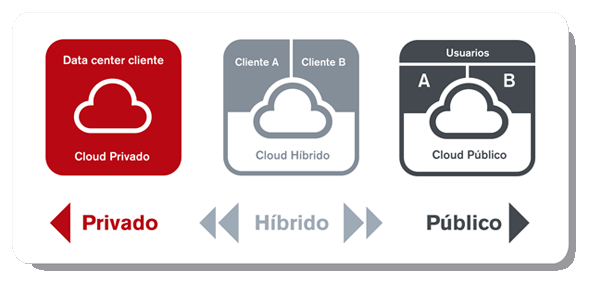
\includegraphics[width=0.7\textwidth]{Imagenes/Bitmap/cloud0}
    \caption{Modelos de despliegue de la computaci\'on en la nube}
    \label{fig:cloud1}
\end{figure}

\subsubsection{Tipos de nubes por el modelo de servicio}
Seg\'un \cite{nist} se ofrecen tres modelos de servicio:
\begin{enumerate}
    \item \textbf{Software as a Service - SaaS}.- Al usuario se le ofrece la
          capacidad de que las aplicaciones  que  su  proveedor  le  suministra
          corran  en  una  infraestructura cloud, siendo las aplicaciones accesibles
          a trav\'es de, por ejemplo, un navegador web como en el caso del webmail,
          que es posiblemente el ejemplo m\'as representativo, por lo extendido,
          de este modelo de servicio. El usuario carece de cualquier control sobre
          la infraestructura o sobre las propias aplicaciones, excepci\'on hecha
          de las posibles configuraciones de usuario o personalizaciones que se
          le permitan.
    \item \textbf{Platform as a Service}.- Al usuario se le permite desplegar
          aplicaciones propias  (ya  sean  adquiridas  o  desarrolladas  por  el
          propio  usuario)  en  la  infraestructura cloud de  su  proveedor, que
          es  quien  ofrece  la  plataforma  de desarrollo y las herramientas de
          programaci\'on. En este caso, es el usuario quien mantiene el control de
          la aplicaci\'on, aunque no de toda la infraestructura subyacente.
    \item \textbf{Infrastructure as a Service}.- El proveedor ofrece al usuario
          recursos como capacidad  de  procesamiento,  de  almacenamiento,  o
          comunicaciones, que el usuario puede utilizar para ejecutar cualquier
          tipo de software, desde sistemas operativos hasta aplicaciones.
\end{enumerate}

\begin{figure}[h]
    \centering
    \captionsetup{justification=centering}
    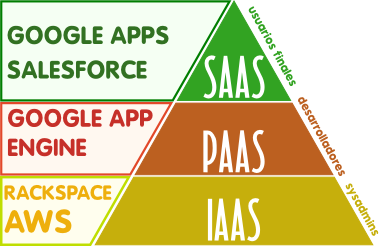
\includegraphics[width=0.7\textwidth]{Imagenes/Bitmap/cloud1}
    \caption{Modelos de servicio de la computaci\'on en la nube con algunos proveedores en cada tipo.}
    \label{fig:cloud1}
\end{figure}

Por otro lado \cite{msolutions} define estos 3 tipos de nubes por el modelo de servicio
de la siguiente forma:
\begin{enumerate}
    \item \textbf{IaaS}: Modelo de servicios en el que al cliente se le ofrece tanto un
          medio de almacenamiento b\'asico como una serie de capacidades de c\'oputo en la red.
          Todo ello haciendo uso de sistemas operativos virtualizados y servidores ubicados
          en la nube a los que el usuario accede a trav\'es de la red.
    \item \textbf{PaaS}: Modelo de servicios en el que al cliente se le ofrece un entorno
          dedicado exclusivamente al desarrollo de aplicaciones. El proveedor de dicho servicio ser\'a
          el encargado de proporcionar la red, los servidores y el almacenamiento necesario.
    \item \textbf{SaaS}: Modelo de servicios en el que al cliente se le proporcionan ciertas aplicaciones
          a trav\'es de Internet. Tanto el \emph{software} como los datos empleados por el usuario
          quedan alojados en los servidores del proveedor de servicios en la nube, accediendo el cliente
          a ellos mediante un navegador web.
\end{enumerate}
\subsubsection{Beneficios de la computaci\'on en la nube}
Respecto a los beneficios de la computaci\'on en la nube \cite{cierco} indica que los beneficios
del cloud son muy relevantes desde distintos puntos de vista.
Para la econom\'ia global, el traslado de las econom\'ias de escala de los
proveedores a las empresas usuarias reduce los costes globales en TI, elimina
las barreras de entrada para nuevos actores y dinamiza la econom\'ia, promoviendo
la aparici\'on de nuevos modelos de negocio y lineas de actividad, facilitando
por la creaci\'on de empresas y de empleo.
%%-------- Servicios web
\subsubsection{Servicios web}

Seg\'un \cite{w3c} define a los servicios web como un sistema de software dise\~nado
para soportar interacci\'on interoperable m\'aquina a m\'aquina a traves de una red.
Por su parte
%%-------- aplicaciones moviles
%%-------- smarth phone
%%-------- Internet
\subsubsection{Internet}
Seg\'un \cite{fnc} Internet hace referencia a un sistema global de informaci\'on que:
\begin{enumerate}[i.]
    \item Esta relacionado l\'ogicamente por un \'unico espacio de direcciones
          global basado en el protocolo de Internet(IP) o en sus extensiones
    \item Es capaz de soportar comunicaciones usando el conjunto de protocolos TCP/IP
          o sus extensiones u otros protocolos compatibles con IP, y
    \item Emplea, provee o hace accesible, privada o p\'ublicamente, servicios de
          alto nivel en capas de comunicaciones y otras infraestructuras relacionadas
          aqui descritas.
\end{enumerate}
%%-------- Intranet
\subsubsection{Intranet}
Seg\'un \cite{lafrance} una Intranet no es m\'as que una Internet privada, interior a una
organizaci\'on y protegida de las miradas indiscretas por una barrera (firewall) que
impide a cualquier intruso conocer su red inform\'atica interna.
%%-------- virtualizacion
%%-------- Digitalizacion
%%-------- Ovicuidad
%%-------- API
%%-------- modelos de negocio en la nube
%%-------- seguridad en la nube
%%-------- tercerizacion u outsourcing
%%-------- riesgos y amenazas
%%-------- SLA
\subsubsection{Acuerdo de nivel de servicio}
Seg\'un \cite{qianq}, un acuerdo de nivel de servicio es usado por las partes
involucradas en un negocio electronico donde los requerimientos minimos y obligaciones son
plasmados en \'el incluyendo los socios de negocio, politica de precios y las propiedad
de los recursos necesarios para la prestacion del servicio de negocio.

Adem\'as \cite{qianq} agrega que los precios parecen ser la caracteristica dominante
de un acuerdo de nivel de servicio, otros asuntos como la disponiblidad, seguridad,
calidad del servicio se convierten en cruciales en este tipo de contratos.

Cabe aclarar que nos podemos referir a estos acuerdos con la abreviatura ANS o SLA,
este ultimo de su traduccion inglesa (Service Layer Agreement).
%%-------- redes sociales

%%-------- Multitenencia
\subsubsection{Multitenencia}

Seg\'un \cite{chandra} la multitenencia es una caracteristicas esencial de los
sistemas en la nube que apunta a proveer aislamiento de diferentes usuarios de
ese sistema en la nube (inquilinos) mientras se maximiza el uso de recursos compartidos.
Adem\'as \citep{chandra} que se espera que esa multitenencia sea soportada en varios niveles de la infraestructura
de la nube, por ejemplo en el nivel de aplicaci\'on, la multitenencia es la que permite
que una sola instancia de una aplicaci\'on pueda escalar para satisfacer a muchos
usuarios al mismo tiempo.

La definci\'on anterior quiere decir que se busca el maximo uso de los recursos
disponibles mientras que los usuarios tengan la sensacion de que usan recursos
independientes.
%%-------- privacidad de los datos
%%-------- seguridad
%%-------- licencia de software
\subsubsection{Licencia de software}
Seg\'un \cite{moro} una licencia de software es un contrato entre el autor o el titular
de los derechos de explotaci\'on de un programa inform\'atico y el usuario (un particular
o una empresa), un contrato que regula los t\'erminos en los que este \'ultimo puede
utilizar el software cumpliento los t\'erminos y las clausulas de la licencia.

Al respecto debemos mencionar que todos las aplicaciones de software tienen una
licencia, algunas de estas licencias son m\'as permisivas que otras. Algunas de estas
son totalmente abiertas (es decir que permiten hacer cualquier cosa con el aplicativo).
%%-------- interoperatividad
\subsubsection{Interoperabilidad}
Seg\'un \cite{kajan} la interoperabilidad es la habilidad de dos o m\'as sistemas o
componentes para intercambiar informaci\'on y usar esa informaci\'on que fue intercambiada.
%%-------- aplicaciones
\subsubsection{Aplicaciones de software}

Seg\'un \cite{pablos} las aplicaciones son programas dise\~nados para ejecutar
trabajos o procesos de c\'alculo espec\'ifico que precisa el usuario o a la unidad
empresarial.
%%-------- migracion a la nube
%%-------- frontend
%%-------- backend
%%-------- internet de las cosas
%%-------- brecha digital
%%-------- aplicaciones web
\subsubsection{Aplicaciones web}
Seg\'un \cite{nino} las aplicaciones web son aplicaciones a las que accede mediante un
navegador y est\'an alojadas en servidores dentro de una Intranet o en Internet.

Adem\'as \cite{nino} agrega que las principales ventajas de las aplicaciones web de
escritorio son:
\begin{itemize}
    \item Se pueden ejecutar desde cualquier equipo inform\'atico siempre que tenga
          una conexi\'on a Internet o a la Intranet.
    \item No es necesario utilizar un sistema operativo en concreto, cualquiera sirve.
    \item No hay que instalar ning\'un programa, con el navegador es suficiente.
    \item No hay que preocuparse del espacio ocupado por los datos, de eso se encarga
          el servidor.
    \item La informaci\'on puede ser compartida simult\'aneamente por .
    \item Se realizan copias de seguridad de la informaci\'on almacenada en el servidor.
    \item Las aplicaciones suelen estar actualizadas en los servidores, algunas
          aplicaciones avisan cuando una actualizaci\'on disponible.
    \item
\end{itemize}

%% ------------------------------- GESTION EMPRESARIAL ------------------------
\subsection{Gesti\'on Empresarial}
\subsubsection{Administraci\'on de empresas}
Seg\'un \cite{koontz} la administraci\'on es el proceso mediante el cual se dise\~na
y mantiene un ambiente en el que individuos que trabajan en grupos cumplen metas
especificas de manera eficaz. Por otra parte \citep{galindo} define la administraci\'on
como el proceso cuyo objeto es la coordinaci\'on eficaz y eficiente de los recursos
de un grupo social para lograr sus objetivos con la m\'axima productividad.
En ambas deficiones se hace hincapi\'e en los terminos eficacia y logro de objetivos
ya que ambos persiguen obtener los mejores resultados posibles con la cantidad
minima de recursos tanto materiales como humanos. Por su parte \citep{chiavenato}
se\~nala que la tarea de la administraci\'on consiste en interpretar los objetivos
de la empresa y transformarlos en acci\'on empresarial mediante planeaci\'on, organizaci\'on,
direcci\'on y control de las actividades realizadas en las diversas \'areas y niveles
de la empresa para conseguir tales objetivos. Por tanto, administraci\'on es el
proceso de planear, organizar, dirigir y controlar el empleo de los recursos
organizacionales para conseguir determinados objetivos con eficiencia y eficacia.

\subsubsection{Proceso administrativo}
\cite{chiavenato} cita a \citep{fayol} quien define el acto de administrar como
\emph{planear, organizar, dirigir, coordinar y controlar}. Las funciones administrativas
abarcan los elementos de la administraci\'on, es decir, las funciones del administrador
(v\'ease la im\'agen \ref{fig:adm}):
\begin{enumerate}
    \item \emph{Planeaci\'on}: avisorar el futuro y trazar el programa de acci\'on.
    \item \emph{Organizaci\'on}: construir las estructuras materiales y sociales de
          la empresa.
    \item \emph{Direcci\'on}: guiar y orientar al personal.
    \item \emph{Coordinaci\'on}: enlazar, unir y armonizar todos los actos y esfuerzos
          colectivos.
    \item \emph{Control}: verificar que todo suceda de acuerdo con las reglas establecidas
          y las \'ordenes dadas.
\end{enumerate}

\subsubsection{Funciones de la empresa}
\cite{chiavenato} cita a \cite{fayol}, indicando que toda empresa cumple seis funciones
(v\'ease la im\'agen \ref{fig:adm}):
\begin{enumerate}
    \item \emph{Funciones t\'ecnicas}, relacionadas con la producci\'on de bienes o
          servicios de la empresa.
    \item \emph{Funciones comerciales}, relacionadas con la compra, la venta o el
          intercambio.
    \item \emph{Funciones financieras}, relacionadas con la b\'usqueda y gesti\'on
          de capitales.
    \item \emph{Funciones de seguridad}, relacionadas con la protecci\'on y preservaci\'on
          de los bienes y las personas.
    \item \emph{Funciones contables}, relacionadas con los inventarios, los registros,
          los balances, los costos y las estad\'isticas.
    \item \emph{Funciones administrativas}, relacionadas con la integraci\'on de las
          otras cinco funciones en la direcci\'on. Las funciones administrativas
          coordinan y sincronizan las dem\'as funciones de la empresa, y est\'an siempre
          por encima de ellas.
\end{enumerate}

\begin{figure}[h]
    \centering
    \captionsetup{justification=centering}
    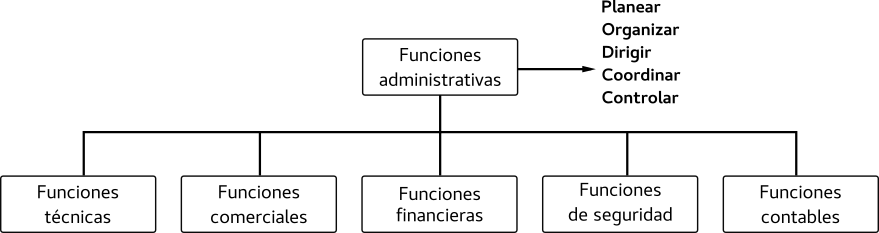
\includegraphics[width=1.0\textwidth]{Imagenes/Bitmap/funciones_adm}
    \caption{Proceso administrativo y funciones de la administraci\'on seg\'un Fayol}
    \label{fig:adm}
\end{figure}

\subsubsection{Gesti\'on}
Seg\'un \cite{beltran} define el termino gesti\'on como el conjunto de decisiones
y acciones que llevan al logro de objetivos previamente establecidos.

Adem\'as \cite{beltran} considera la gesti\'on en tres niveles diferentes:
\begin{enumerate}
    \item \textbf{Gesti\'on estrat\'egica}: Se desarrolla en la direcci\'on, y tiene como
          caracter\'istic fundamental que la influencia de las acciones y las decisiones
          es, generalmente, corporativa y de largo plazo.
    \item \textbf{Gesti\'on t\'actica}: Se desarrolla con base en la gesti\'on
          estrat\'egica. El impacto de las decisiones y acciones, de mediano plazo,
          abarca las unidades estrat\'egicas del negocio.
    \item \textbf{Gesti\'on operativa}: Se desarrolla con base en la gesti\'on
          t\'actica. El impacto de la decisiones y acciones es de corto plazo e incluye
          los equipos naturales de trabajo y los individuos. B\'asicamente tiene
          que ver con la funciones de ejecuci\'on y control.
\end{enumerate}

\subsubsection{Control de gesti\'on}
% TODO : Citar a la fuente original
Seg\'un \cite{beltran} el control de gesti\'on es un instrumento gerencial, integral
y estrat\'egico que, apoyado en indicadores, \'indices y cuadros producidos en forma
sistem\'atica, peri\'odica y objetiva, permite que la organizaci\'on sea efectiva para
captar recursos, eficiente para transformarlos y eficaz para canalizarlos.

Por otro lado, \cite{beltran} agrega que un sistema de control de gesti\'on tiene
como objetivo facilitar a los administradores con responsabildades de planeaci\'on
y control de cada grupo operativo, informaci\'on permanente e integral sobre su desempe\~no,
que les permita a \'estos autoevaluar su gesti\'on y tomar los correctivos del caso.

\subsubsection{Indicadores de gesti\'on}
Previamente \cite{beltran} define indicador coo la relaci\'on entre las variables
cuantitativas o cualitativas que permiten observar la situaci\'on y las tendencias
de cambio generadas en el objeto o fen\'omeno observado, respecto de los objetivos
y metas previstos e influencias esperadas.

Respecto a esto \cite{silva} agrega que uno de los objetivos principales de los
indicadores de gesti\'on consiste en establecer un sistema de instrumentos que
permita en forma r\'apida y proactiva, administrar la empresa y hacer posible la
comparaci\'on de los resultados con la metas propuestas y de igual forma definir
par\'ametros que permitan que el dise\~no de los objetivos, los planes y las metas sean
reales en el tiempo para controlar las operaciones diarias que se realizan dentro
de la empresa. Tambi\'en crear mecanismos de detecci\'on de fallas que garanticen
la posibilidad de llevar a cabo acciones concretas que permitan obtener soluciones
reales y de aplicaci\'on inmediata.

Seg\'un \cite{beltran}, los indicadores de gesti\'on son, ante todo, informaci\'on, es
decir, agregan valor, no son solo datos. Siendo informaci\'on, los indicadores de
gesti\'on deben tener los atributos de la informaci\'on, tanto en forma individual
como cuando se presentan agrupados.

En los parrafos anteriores queda de manifiesto la importancia de los indicadores
de gesti\'on como instrumentos que permiten determinar la situaci\'on actual de la
empresa en distintos aspectos y a la vez permiten fijar las estrategias futuras
para que estas sean alcanzables en el tiempo.

\subsubsection{Caracter\'isticas de los indicadores}
Seg\'un \cite{silva} los indicadores de gesti\'on deben cumplir con unos requisitos
y elementos para poder apoyar la gesti\'on para conseguir el objetivo, las cuales
pueden ser:
\begin{enumerate}
    \item \emph{Simplicidad}, se puede entender como la capacidad para definir el
          evento que se pretende medir de manera poco costosa en tiempo y recurso.
    \item \emph{Validez en el tiempo}, Puede definirse como la propiedad de ser
          permanente en un periodo deseado.
    \item \emph{Adecuaci\'on}, Corresponde a la facilidad de la medida para describir
          por completo el fen\'omeno o efecto. Debe reflejar la magnitud del hecho
          analizado y mostrar la desviaci\'on real del nivel deseado.
    \item \emph{Utilidad}, es la posibilidad del indicador para estar siempre
          orientado a buscar las causas que han llevado a que alcance un valor
          particular y mejorarlas.
    \item \emph{Participaci\'on de los usuarios}, es la habilidad para estar involucrados
          desde el dise\~no, y debe proporcionarseles los recursos y formaci\'on necesarios
          para su ejecuci\'on.
    \item \emph{Oportunidad}, es la capacidad para que los datos sean recolectados
          a tiempo, igualmente se requiere que la informaci\'on sea analizada oportunamente
          para poder actual.
\end{enumerate}

\subsubsection{Indicadores del negocio con base en el esquema de valor de negocio}
Seg\'un \cite{cruz} para la identificaci\'on de variables e indicadores del negocio
se considera inicialmente el ESQUEMA DE VALOR DE MERCADO, los cuales est\'an asociados
generalmente con la misi\'on y sus elementos cuantificables como de las estrategias,
y luego son transformados en indicadores b\'asicos, clave y operativos.

Adem\'as \cite{cruz} agrega que el esquema de valor de mercado de una empresa est\'a
soportado por cuatro (4) grandes macroindicadores: rentabilidad, competitividad,
riesgo y liquidez. Todos ellos, excepto el riesgo, son de signo creciente, es
decir mejoran al crecer de valor.

\begin{figure}[t]
    \begin{center}
        \includegraphics[width=1.0\textwidth]%
        {Imagenes/Vectorial/valor}
        \caption{Esquema de valor de mercado}
        \label{fig:indicadores_valor_mercado}
    \end{center}
\end{figure}

\subsubsection{Indicador de Efectividad}
Seg\'un \cite{cruz} la efectividad, significa cuantificaci\'on del logro de la meta,
tambi\'en es sin\'onimo de eficacia y se le define como \emph{Capacidad de lograr el
efecto que se desea}. Los indicadores de eficacia o efectividad, tienen que ver
con hacer realidad un intento o prop\'osito, y est\'an relacionados con el cumplimiento
al ciento por ciento de los objetivos planteados.

\cite{cruz} ubica a la efectividad respecto a los indicadores del negocio con base
en el esquema de valor de mercado de la figura \ref{fig:indicadores_valor_mercado}
como parte de la Rentabilidad, tal como se puede ver en la figura \ref{fig:efectividad}

Adem\'as \cite{cruz} se\~nala que se pueden dise\~nar indicadores de efectividad
como el de las formulas \ref{eq:calc_efectividad_instalaciones} y \ref{eq:calc_efectividad_ventas}
pero \'estos no son \'unicos.

\begin{figure}[t]
    \begin{center}
        \includegraphics[width=0.8\textwidth]%
        {Imagenes/Vectorial/efectividad}
        \caption{Efectividad}
        \label{fig:efectividad}
    \end{center}
\end{figure}

\begin{equation}\label{eq:calc_efectividad_instalaciones}
\text{Efectividad en las instalaciones} = \frac{\text{Vol}_{\text{producido}}}{\text{Vol}_{\text{programado}}} \times{100}
\end{equation}

\begin{equation}\label{eq:calc_efectividad_ventas}
\text{Efectividad en ventas} = \frac{\text{Vol}_{\text{vendido}}}{\text{Vol}_{\text{planificado}}} \times{100}
\end{equation}

\cite{cruz} agrega la especificaci\'on de los indicadores de efectividad mostradolos
en la tabla \ref{t:efectividad}.

\begin{table}
    \begin{tabular}{|p{8cm}|p{5cm}|}
        \hline
        \thead{Descripci\'on del Indicador} & \thead{Variables fundamentales} \\ \hline
        \begin{minipage}{3in}
            \textbf{Efectividad en el uso de instalaciones}\\
            Es el grado de cumplimiento del programa de
            producci\'on. Este factor puede estar afectado por
            causas imputadas tanto a los equipos de producci\'on, como a los que administran el proceso. El
            indicador es medido porcentualmente ( \%).
        \end{minipage}
         &
        \begin{minipage}{2in}
            \vskip 4pt
            \begin{enumerate}
                \item Disponibilidad de las instalaciones.
                \item Eficiencia de los equipos.
                \item Efectividad en la logistica y transporte.
            \end{enumerate}
            \vskip 4pt
        \end{minipage}
        \\
        \hline
        \begin{minipage}{3in}
            \textbf{Efectividad en las ventas}\\
            Es el grado de cumplimiento del plan de ventas, en t\'erminos de
            volumen despachado, tanto para el mercado nacional como para
            exportaci\'on, as\'i como el total. El indicador es medido
            porcentualmente (\%).
        \end{minipage}
         &
        \begin{minipage}{2in}
            \vskip 4pt
            \begin{enumerate}
                \item Efectividad en el uso de las instalaciones.
                \item Eficiencia en la gesi\'on de comercializaci\'on y ventas.
            \end{enumerate}
            \vskip 4pt
        \end{minipage}
        \\
        \hline
    \end{tabular}
    \caption{Especificaci\'on de los indicadores de efectividad}
    \label{t:efectividad}
\end{table}

\subsubsection{Indicador de eficiencia}
Seg\'un \cite{cruz} la eficiencia es la capacidad administrativa de producir el
m\'aximo de resultados con el m\'inimo de recursos, el m\'inimo de energ\'ia y en el
m\'inimo de tiempo posible.

\cite{cruz}, tambien muestra la relacion de la eficiencia y la rentabilidad de la
figura \ref{fig:indicadores_valor_mercado} por medio de la figura \ref{fig:eficiencia}.

Adem\'as \cite{cruz} indica que entre los indicadores de eficiencia se pueden
mencionar los de las ecuaciones \ref{eq:calc_eficiencia_capacidad_instalada}, \ref{eq:calc_eficiencia_capacidad_instalada}

\begin{figure}[t]
    \begin{center}
        \includegraphics[width=0.7\textwidth]%
        {Imagenes/Vectorial/eficiencia}
        \caption{Eficiencia}
        \label{fig:eficiencia}
    \end{center}
\end{figure}

\begin{equation}\label{eq:calc_eficiencia_capacidad_instalada}
    \text{Uso de la capacidad instalada}=\frac{\text{Volumen de producci\'on}}{\text{Capacidad instalada}} \times{100}
\end{equation}

\begin{equation}\label{eq:calc_eficiencia_capacidad_instalada}
    \text{Nivel de inventarios}=\frac{\text{Costo del inventario}}{\text{Ventas netas}} \times{100}
\end{equation}

Adem\'as \cite{cruz} muestra la especificaci\'on del indicador mencionando su
descripci\'on y sus variables en la tabla \ref{t:eficiencia}.

\begin{table}
    \begin{tabular}{|p{5cm}|p{8cm}|}
        \hline
        \thead{Descripci\'on del Indicador} & \thead{Variables fundamentales} \\ \hline
        \begin{minipage}{2in}
            \textbf{Uso de la capacidad instalada}\\
            Indica el uso racional de las instalaciones productivas, con base en
            la capacidad nominal o instalada. El indicador es medido porcentualmente (\%).
        \end{minipage}
         &
        \begin{minipage}{3in}
            \vskip 4pt
            \begin{enumerate}
                \item Disponibilidad de las instalaciones.
                \item Eficiencia en el mantenimiento.
                \item Efectividad en el transporte.
                \item Capacidad de las instalaciones.
            \end{enumerate}
            \vskip 4pt
        \end{minipage}
        \\
        \hline
        \begin{minipage}{2in}
            \textbf{Nivel de inventarios}\\
            Permite conocer el uso racional del capital invertido en inventarios
            con relaci\'on a las ventas netas. El indicador es medido porcentualmente (\%).
        \end{minipage}
         &
        \begin{minipage}{3in}
            \vskip 4pt
            \begin{enumerate}
                \item Eficiencia en el uso de los insumos.
                \item Determinaci\'on optima de los niveles de reposici\'on.
                \item Efectividad en el pago a proveedores.
                \item Eficiencia en el tiempo de compras.
            \end{enumerate}
            \vskip 4pt
        \end{minipage}
        \\
        \hline
    \end{tabular}
    \caption{Especificaci\'on de los indicadores de eficiencia}
    \label{t:eficiencia}
\end{table}

\subsubsection{Indicador de calidad}
Seg\'un \cite{cruz} el concepto t\'ecnico de calidad representa m\'as bien una forma
de hacer las cosas en las que, fundamentalmente, predominan la preocupaci\'on por
satisfacer al cliente y por mejorar, d\'ia a d\'ia, procesos y resultados. Hoy en d\'ia
introduce el concepto de mejora continua en cualquier organizaci\'on y a todos los
niveles de la misma. Entre los indicadores de eficiencia se pueden mencionarlos
siguientes:

\begin{figure}[t]
    \begin{center}
        \includegraphics[width=0.7\textwidth]%
        {Imagenes/Vectorial/calidad}
        \caption{Calidad}
    \end{center}
\end{figure}

\begin{equation}\label{eq:rendimiento_calidad}
    \text{Rendimiento de calidad}=\frac{\text{Vol}_{\text{producci\'on conforme}}}{\text{Vol}_{\text{total producido}}} \times{100}
\end{equation}

\begin{equation}\label{eq:calidad_uso}
    \text{Calidad de uso}=\frac{\text{Volumen reclamado por calidad (procedente)}}{\text{Volumen total de ventas}} \times{100}
\end{equation}

\begin{table}
    \begin{tabular}{|p{5cm}|p{8cm}|}
        \hline
        \thead{Descripci\'on del Indicador} & \thead{Variables fundamentales} \\ \hline
        \begin{minipage}{2in}
            \textbf{Relaci\'on deuda/calidad}\\
            Mide el nivel de apalancamiento del negocio, con recursos externos
            con base en el patrimonio. El indicador es medido porcentualmente (\%).
        \end{minipage}
         &
        \begin{minipage}{3in}
            \vskip 4pt
            \begin{enumerate}
                \item Efectividad en el uso de las instalaciones.
                \item Tiempo efectivo de trabajo.
                \item Cumplimiento plan de desarrollo y capacitaci\'on.
                \item Eficiencia en la gesti\'on de calidad.
            \end{enumerate}
            \vskip 4pt
        \end{minipage}
        \\
        \hline
    \end{tabular}
    \caption{Especificaci\'on de los indicadores de calidad}
    \label{t:calidad}
\end{table}

\subsubsection{Indicador de productividad}
Seg\'un \cite{cruz} los indicadores de productividad son los siguientes:

\begin{figure}[t]
    \begin{center}
        \includegraphics[width=1.0\textwidth]%
        {Imagenes/Vectorial/productividad}
        \caption{Productividad}
    \end{center}
\end{figure}

\begin{equation}\label{eq:productividad_mano_obra}
    \text{Productividad de mano de obra}=\frac{\text{Vol}_{\text{producci\'on conforme}}}{\text{Horas hombre trabajadas}}
\end{equation}

\begin{equation}\label{eq:productividad_costo_unitario}
    \text{Costo Unitario de Producci\'on} = \frac{\text{Costo total de producci\'on}}{\text{Volumen de producci\'on conforme}}
\end{equation}

\begin{equation}\label{eq:productividad_capital}
    \text{Productividad del capital} = \frac{\text{Volumen de producci\'on conforme}}{\text{Activo total promedio}}
\end{equation}

\begin{table}
    \begin{tabular}{|p{7cm}|p{7cm}|}
        \hline
        \thead{Descripci\'on del Indicador} & \thead{Variables fundamentales} \\ \hline
        \begin{minipage}{2.5in}
            \textbf{Rentabilidad total}\\
            Es la rentabilidad medida en t\'erminos de la capacidad de generar
            utilidades con los activos disponibles. El indicador es medido
            porcentualmente (\%). \\
            \textbf{Margen neto}\\
            Mide la rentabilidad en funci\'on de las ventas generadas. El
            indicador es medido porcentualmente (\%). \\
            \textbf{Rotaci\'on del activo} \\
            Mide las veces que en un a\~no se mueve el activo de la empresa y
            muestra la intensidad con que los activos totales se est\'an utilizando.\\
            \textbf{Margen de operaciones} \\
            Mide las ganancias en operaciones en funci\'on de las ventas generadas,
            sin tomar en cuenta la carga financiera y los impuestos. El indicador
            es medido porcentualmente (\%).
        \end{minipage}
         &
        \begin{minipage}{2.5in}
            \vskip 4pt
            \begin{enumerate}
                \item Cumplimiento del Plan de Ventas.
                \item Efectividad en el Plan de Producci\'on.
                \item Cumplimiento en la ejecuci\'on presupuestaria.
                \item Eficiencia en el uso de los recursos.
                \item Eficiencia en la gesti\'on de comercializaci\'on y ventas.
                \item Control efectivo de los activos y pasivos.
                \item Administraci\'on de los programas de reducci\'on de costos.
                \item Eficiencia en la gesti\'on de calidad.
            \end{enumerate}
            \vskip 4pt
        \end{minipage}
        \\
        \hline
    \end{tabular}
    \caption{Especificaci\'on de los indicadores de rentabilidad}
    \label{t:rentabilidad}
\end{table}

\subsubsection{Indicador de apalancamiento}
Seg\'un \cite{cruz} los indicadores de apalancamiento son los siguientes:

\begin{figure}[t]
    \begin{center}
        \includegraphics[width=1.0\textwidth]%
        {Imagenes/Vectorial/apalancamiento}
        \caption{Apalancamiento}
    \end{center}
\end{figure}

\begin{equation}\label{apalancamiento}
    \text{Relaci\'on deuda/capital} = \frac{\text{Deuda total}}{\text{Patrimonio}}\times{100}
\end{equation}

\subsubsection{Indicadores de rentabilidad}
Seg\'un \cite{cruz} los indicadores de rentabilidad son:

\begin{figure}[t]
    \begin{center}
        \includegraphics[width=1.0\textwidth]%
        {Imagenes/Bitmap/rentabilidad01}
        \caption{Rentabilidad}
    \end{center}
\end{figure}

\begin{equation}\label{eq:rentabilidad_total}
    \text{Rentabilidad total}=\frac{\text{Utilidad total}}{\text{Activo total promedio}}\times{100}
\end{equation}

\begin{equation}\label{eq:margen_neto}
    \text{Margen neto}=\frac{\text{Utilidad neta}}{\text{Ventas netas}}\times{100}
\end{equation}

\begin{equation}\label{eq:rotacion_activo}
    \text{Rotaci\'on del activo (veces)}=\frac{\text{Ventas netas}}{\text{Activo total promedio}}
\end{equation}

\begin{equation}\label{eq:margen_operaciones}
    \text{Margen operaciones} = \frac{\text{Utilidad en operaciones}}{\text{Ventas netas}}\times{100}
\end{equation}

\begin{table}
    \begin{tabular}{|p{5cm}|p{7.5cm}|}
        \hline
        \thead{Descripci\'on del Indicador} & \thead{Variables fundamentales} \\ \hline
        \begin{minipage}{2in}
            \textbf{Riesgo operativo}\\
            Posibilidad de no estar en capacidad de cubrir los costos de operaci\'on.
            Tambi\'en mide el peligro de no ganar. \\
            \textbf{Riesgo financiero}\\
            Posibilidad de no estar en condiciones de cubrir los costos de financieros,
            o sea mide el peligro a que est\'a expuesta la empresa de no pagar sus deudas. \\
        \end{minipage}
         &
        \begin{minipage}{3in}
            \vskip 4pt
            \begin{enumerate}
                \item Cumplimiento del Plan de Ventas.
                \item Efectividad en el Plan de Producci\'on.
                \item Cumplimiento en la ejecuci\'on presupuestaria.
                \item Eficiencia en el uso de los recursos.
                \item Eficiencia en la gesti\'on de comercializaci\'on y ventas.
                \item Administraci\'on de los programas de reducci\'on de costos.
                \item Eficiencia en la gesti\'on de calidad.
            \end{enumerate}
            \vskip 4pt
        \end{minipage}
        \\
        \hline
    \end{tabular}
    \caption{Especificaci\'on de los indicadores de riesgo}
    \label{t:riesgo}
\end{table}

\subsubsection{Indicadores de riesgo}
\cite{cruz} indica que si la empresa no cotiza en la bolsa y sus acciones no tienen
variabilidad estad\'istica, por supuesto, no se tienen los soportes para calcular
los indicadores de riesgo, pero no implica que no tengan riesgos, por lo tanto
es posible establecer un indicador de riesgo empresarial, entendiendo por este
la posibilidad de que la organizaci\'on no pueda cubrir sus costos de operaci\'on
y/o financieros.

En este sentido \cite{cruz} se\~nala que el indicador tiene su base en las
utilidades antes de intereses e impuestos que pueda tener la empresa, a fin de
cubrir sus costos de operaci\'on (fijos y variables) y las utilidades antes de
impuestos, a fin de cubrir sus costos financieros.

En este sentido \cite{cruz} distingue dos tipos de riesgos:
\begin{itemize}
    \item \emph{RIESGO OPERATIVO}, posibilidad de no estar en capacidad de cubrir
          los costos de operaci\'on. Tambi\'en mide el peligro de no ganar en las
          operaciones.
    \item \emph{RIESGO FINANCIERO}, posibilidad de no estar en condiciones de
          cubrir los costos de financieros, o sea mide el peligro a que est\'a
          expuesta la empresa de no pagar sus deudas.
\end{itemize}

Dado esto \cite{cruz} establece indicadores de riesgo operativo y financiero en las
formulas \ref{eq:riesgo1} y \ref{eq:riesgo2}.

\begin{equation}\label{eq:riesgo1}
    \text{Riesgo operativo} = \text{Utilidad en operaciones} \geq 0
\end{equation}

\begin{equation}\label{eq:riesgo2}
    \text{Riesgo financiero} = \text{Utilidad antes de impuestos} \geq 0
\end{equation}

\subsubsection{Indicadores de competitividad}
Seg\'un \cite{cruz} se entiende por competitividad a la capacidad de una organizaci\'on
p\'ublica o privada, lucrativa o no, de mantener sistem\'aticamente ventajas comparativas
que le permitan alcanzar, sostener y mejorar una determinada posici\'on en el entorno
socioecon\'omico.

\cite{cruz} define los indicadores en las formulas \ref{eq:competitividad1} y
\ref{eq:competitividad2}.

\begin{equation}\label{eq:competitividad1}
    \text{Comp. CU del producto} = \frac{\text{Costo producto propio}}{\text{Costo producto competidor}} \times{100}
\end{equation}

\begin{equation}\label{eq:competitividad2}
    \text{Var. participaci\'on en mercado} = \frac{\text{Participaci\'on a\~no anterior}}{\text{Participaci\'on a\~no actual}}\text{100}
\end{equation}

%\subsubsection{Liquidez}
%\subsubsection{mipyme}
%\subsubsection{emprendimiento}
\newpage
\section{Hip'otesis}

\subsection{Hip'otesis General}

Existe un efecto positivo del uso de la computaci\'on en la nube en la
gesti'on de las micro, peque\~nas y medianas empresas pertenecientes al Centro de
Desarrollo Empresarial del Cusco.

\subsection{Hip'otesis Espec'ificas}
\begin{enumerate}[a., noitemsep]
    % preguntaar si es necesario colocar las palabras pe-post implementacion
    \item El nivel de gesti\'on de las MiPYMES pertenecientes al Centro de Desarrollo
          Empresarial del Cusco antes del uso de las herramientas de la computaci\'on
          en la nube es deficiente.
    \item El nivel de gesti\'on de las MiPYMES pertenecientes al Centro de Desarrollo
          Empresarial del Cusco despu\'es del uso de las herramientas de la computaci\'on
          en la nube es eficiente.
    \item El efecto del uso de herramientas de la computaci'on en la nube en la
          gesti\'on de las MiPYMES pertenecientes al Centro de Desarrollo Empresarial
          del Cusco es positiva.
\end{enumerate}

\section{Variables}

\subsection{Identificaci'on de variables}

\begin{enumerate}[a., noitemsep]
    \item Uso de aplicaciones del modelo Software como Servicio.
    \item Gesti\'on Empresarial.
\end{enumerate}

%-----------------
\subsection{Operacionalizaci'on de variables}
El proceso de operacionalizaci\'on de variables se realizo basicamente analizando dos variables:
\begin{itemize}[noitemsep]
    \item El uso de aplicaciones del modelo Software como Servicio.
    \item La gesti\'on empresarial.
\end{itemize}
El an\'alisis de la primera variable se muestra en la tabla \ref{t_saas}, mientras
que el an\'alisis de la segunda variable se muestra en la tabla \ref{t:gestion}.

\begin{sidewaystable}[]
    \caption{Operacionalizaci\'on de la variable ``\emph{Uso de aplicaciones del modelo Software como Servicio}''}
    \label{t_saas}
    \centering
    \begin{tabular}{|p{3cm}|p{4cm}|p{3.5cm}|p{3.5cm}|p{5cm}|}
    \hline
    \thead{Variables} & \thead{Definici\'on \\ Conceptual} & \thead{Definici\'on \\ Operacional} & \thead{Dimensiones} & \thead{Indicadores} \\ \hline
    \multirow{5}{3cm}{Uso de aplicaciones del modelo Software como Servicio} &
    \multirow{5}{4cm}{El software como servicio (SaaS) se puede describir sucintamente
                 como el software que se despliega en un servicio alojado y se puede
                 acceder globalmente a trav\'es de Internet, la mayor\'ia de las veces
                 en un navegador. Con la excepci\'on de la interacci\'on del usuario
                 con el software, todos los dem\'as aspectos del servicio se abstraen\citep{sosinsky}.} &
    \multirow{5}{3.5cm}{El modelo SaaS se basa en la aplicaci\'on pr\'actica que tiene
                 para una organizaci\'on el hecho de que sus empleados o clientes
                 puedan acceder a una aplicaci\'on sin necesidad de instalarla en
                 sus dispositivos\citep{msolutions}.} &
     Disponibilidad de equipos inform\'aticos. &
     \begin{itemize}[noitemsep]
         \item Inventario de equipos de computo.
         \item Inventario de equipos moviles (tablets y celulares).
         \item Capacidad de los equipos para procesar informaci\'on y navegar por Internet.
     \end{itemize}
      \\ \cline{4-5}
     &  &  & Conectividad. &
     \begin{itemize}[noitemsep]
         \item Presencia de conexi\'on a Internet.
         \item Tipo de conexi\'on utilizada.
         \item Capacidad de la conexi\'on utilizada.
         \item Tipo de uso de la conexi\'on disponible.
     \end{itemize}  \\ \cline{4-5}
     &  &  & Disponibilidad de sistemas de informaci\'on/gesti\'on. &
     \begin{itemize}[noitemsep]
         \item Tipo de sistemas de informaci\'on / gesti\'on utilizados.
         \item Origen de los sistemas de informaci\'on / gesti\'on utilizados.
         \item Costo de los sistemas de informaci\'on / gesti\'on utilizados.
     \end{itemize} \\ \hline
    \end{tabular}
\end{sidewaystable}
%%---
\begin{sidewaystable}[htbp]
    \centering
    \caption{Operacionalizaci\'on de la variable ``\emph{Gesti\'on empresarial}''}
    \label{t:gestion}
    \begin{tabular}{|p{3cm}|p{4cm}|p{3.5cm}|p{3.5cm}|p{5cm}|}
    \hline
    \thead{Variable} & \thead{Definici\'on\\Conceptual} & \thead{Definici\'on\\Operacional} & \thead{Dimensiones} & \thead{Indicadores} \\ \hline
    \multirow{1}{3cm}{Gesti\'on empresarial} &
    \multirow{5}{4cm}{La administraci\'on es el proceso mediante el cual se dise\~na
            y mantiene,un ambiente, en el que individuos que trabajan en grupos,
            cumplen metas,especificas de manera eficaz\citep{koontz}} &
    \multirow{5}{3.5cm}{Seg\'un \cite{fayol} toda empresa posee seis funciones b\'asicas:} &
    Producci\'on &
    \begin{itemize}[noitemsep]
      \item Uso de insumos / materia prima.
      \item Cantidad de productos producidos.
    \end{itemize} \\ \cline{4-5}
     &  &  & Comercializaci\'on &
     \begin{itemize}[noitemsep]
       \item Cantidad de ventas.
       \item Registro de clientes.
       \item Registro de proveedores.
     \end{itemize} \\ \cline{4-5}
     &  &  & Administraci\'on &
     \begin{itemize}[noitemsep]
       \item Ingresos y egresos.
       \item Flujo de efectivo.
     \end{itemize} \\ \hline
    \end{tabular}
\end{sidewaystable}

\section{Definici\'on de t\'erminos b\'asicos}

La definici\'on de t\'erminos b\'asicos se encuentran en la tabla \ref{t:glosario}
\begin{table}[htbp]
    \centering
    \caption{Definici\'on de t\'erminos b\'asicos}
    \label{t:glosario}
    \begin{tabular}{|p{3cm}|p{8cm}|}
    \hline
    \thead{Termino} & \thead{Definici\'on} \\ \hline
    Software como Servicio & El software como servicio (SaaS) se puede describir sucintamente,como el software que se despliega en un servicio alojado y se puede,acceder globalmente a trav\'es de Internet, la mayor\'ia de las veces,en un navegador. Con la excepci\'on de la interacci\'on del usuario,con el software, todos los dem\'as aspectos del servicio se abstraen\citep{sosinsky}. \\ \hline
    Gesti\'on empresarial & La administraci\'on es el proceso mediante el cual se dise\~na,y mantiene,un ambiente, en el que individuos que trabajan en grupos,,cumplen metas,especificas de manera eficaz\citep{koontz} \\ \hline
    \end{tabular}
\end{table}

%---------------------------------------------------------------------
%                          Capítulo 3
%---------------------------------------------------------------------

\chapter{Método}
\section{Alcance del Estudio}
En palabras de \cite{sampieri}, el alcance del estudio es importante por que de
ésta dependera la estrategia de la investigación y como consecuencia el diseño,
procedimientos y otros componentes del proceso serán distintos de acuerdo al alcance
planteado.

De acuerdo a \cite{sampieri} existen 4 tipos de alcance, los cuales son:
\begin{itemize}
    \item \textbf{Exploratorios}, utilizados en problemas poco estudiados, indagan
          desde una perspectiva innovadora, ayudan a identificar conceptos promisorios,
          preparan el terreno para nuevos estudios.
    \item \textbf{Descriptivos}, consideran al fenómeno estudiando y sus componentes,
          miden conceptos y definen variables.
    \item \textbf{Correlacionales}, asocian conceptos o variables, permiten predicciones,
          cuantifican relaciones entre conceptos o variables.
    \item \textbf{Explicativos}, determinan las causas de los fénomenos, generan un
          sentido de entendimiento, son sumamente estructurados.
\end{itemize}

El estudio que se realizará en el Centro de Desarrollo Empresarial del Cusco será
de \textbf{alcance explicativo}, debido a que se pretende determinar si el uso
de herramientas de la computación en la nube, especificamente el modelo de
\emph{Software como Servicio}, ayuda a mejorar la gestión empresarial de las empresas
beneficiarias del Centro de Desarrollo Empresarial del Cusco.

\section{Diseño de investigación}
En palabras de \cite{sampieri}, la gestación del diseño del estudio representa
el punto donde se conectan las etapas conceptuales del proceso de investigación
como el planteamiento del problema, el desarrollo de la perspectiva teórica y
la hipótesis con las fases subsecuentes cuyo carácter es más operativo.

Además \cite{sampieri} agrega que el propósito del diseño de investigación
es:
\begin{itemize}
    \item Responder preguntas de investigación.
    \item Cumplir objetivos del estudio.
    \item Someter hipótesis a prueba.
\end{itemize}

Respecto a los tipos de diseños disponibles, \cite{sampieri} indica que existen
dos tipos principales: investigación experimental e investigación no experimental.
A su vez, la primera puede dividirse de acuerdo con las clásicas categorías de
Campbell y Stanley (1966) en: preexperimentos, experimentos ``puro'' y cuasiexperimentos.
La investigación no experimental la subdividimos en diseños transversales y diseños
longitudinales.

\cite{sampieri} señala respecto a los \emph{preexperimentos} que se denominan de
esa forma debido a que su grado de control es mínimo. Se caracteriza por investigar
un solo grupo cuyo grado de control es mínimo. Generalmente es útil como primer
acercamiento al problema de investigación en la realidad.

Debido a que el enfoque para este trabajo es cuantitativo, se deberá realizar
una \textbf{investigación experimental} siendo el tipo específico la \textbf{preexperimental}.

\section{Población}
% TODO: Definir tacitamente que es el CDE (definicion formal o legal) y complementar
% esta sección
Como se menciono en secciones anteriores, el trabajo de investigación se realizará
con la empresas que son beneficiarias del Centro de Desarrollo Empresarial del Cusco,
constituido en la ciudad del Cusco por convenio entre el CEC Guaman Poma de Ayala
y el Ministerio de la Producción.

En este caso no se tomarán muestras sino que se considerará la población de
empresas en todo su conjunto debido a que la cantidad es pequeña, aproximadamente
30 empresas.

\section{Técnicas e instrumentos de recolección de datos}
Según \cite{robledo} en función de las distintas técnicas que se aplican para
la obtención de los datos o evidencias, se distinguen tres áreas las cuales son:
\begin{itemize}
    \item Investigación documental.
    \item Investigación de campo.
    \item Investigación de laboratorio,.
\end{itemize}

La investigación documental consiste en la recolección de información ya existente
que este debidamente documentada, según \cite{robledo} agrega que en este tipo
de investigación se distinguen distintos instrumentos, haciendo hincapié en las
\emph{fichas}, las cuales \citep{robledo} las clasifica en:
\begin{itemize}
    \item Fichas bibliograficas.
    \item Fichas de trabajo.
\end{itemize}

Respecto a las fichas de trabajo \cite{robledo} indica que es el instrumento de
trabajo intelectual que se utiliza para recabar, registrar, clasificar y
manejar los datos relacionados con un problema de investigación.

Bajo este entender, las técnicas que se aplicarán para este trabajo serán:
la \textbf{investigación documental} e \textbf{investigación de campo} utilizando
como instrumentos especificos las \textbf{fichas de trabajo} y \textbf{encuestas}.

\section{Validez y confiabilidad de instrumentos}

\section{Plan de Análisis de datos}
Para el análisis de datos se utilizará la \textbf{Prueba T de Student, Prueba
T-Student o Test-T}, ya que es la que más se adecua a nuestro escenario.

%---------------------------------------------------------------------
%                          Cap\'itulo 4
%---------------------------------------------------------------------
\chapter{Aspectos operativos}
\section{Cronograma}
\begin{ganttchart}[
    canvas/.append style={fill=none, draw=black!5, line width=.75pt},
    hgrid style/.style={draw=black!5, line width=.75pt},
    vgrid={*1{draw=black!5, line width=.75pt}},
    today=7,
    today rule/.style={
      draw=black!64,
      dash pattern=on 3.5pt off 4.5pt,
      line width=1.5pt
    },
    today label font=\small\bfseries,
    title/.style={draw=none, fill=none},
    title label font=\bfseries\footnotesize,
    title label node/.append style={below=7pt},
    include title in canvas=false,
    bar label font=\mdseries\small\color{black!70},
    bar label node/.append style={left=2cm},
    bar/.append style={draw=none, fill=black!63},
    bar incomplete/.append style={fill=barblue},
    bar progress label font=\mdseries\footnotesize\color{black!70},
    group incomplete/.append style={fill=groupblue},
    group left shift=0,
    group right shift=0,
    group height=.5,
    group peaks tip position=0,
    group label node/.append style={left=.6cm},
    group progress label font=\bfseries\small,
    link/.style={-latex, line width=1.5pt, linkred},
    link label font=\scriptsize\bfseries,
    link label node/.append style={below left=-2pt and 0pt}
  ]{1}{13}
  [grid]
  \ganttbar[name=WBS1A]{1. B\'usqueda de tema}{1}{8} \\
  \ganttbar[name=WBS1A]{2. Definici\'on de tema}{1}{8} \\
  \ganttbar[name=WBS1A]{3. Planteamiento del problema}{1}{8} \\
  \ganttbar[name=WBS1A]{4. B\'usqueda de fuentes de informaci\'on}{1}{8} \\
  \ganttbar[name=WBS1A]{5. Elaboraci\'on del proyecto}{1}{8} \\
  \ganttbar[name=WBS1A]{6. Construcci\'on del marco te\'orico}{1}{8} \\
  \ganttbar[name=WBS1A]{7. Redacci\'on del proyecto de investigaci\'on}{1}{8} \\
  \ganttbar[name=WBS1A]{8. Construcci\'on  de los instrumentos de elaboraci\'on}{1}{8} \\
  \ganttbar[name=WBS1A]{9. Aplicaci\'on del trabajo de campo}{1}{8} \\
  \ganttbar[name=WBS1A]{10. Observaci\'on de la muestra}{1}{8} \\
  \ganttbar[name=WBS1A]{11. An\'alisis de datos}{1}{8} \\
  \ganttbar[name=WBS1A]{12. Redacci\'on del primer borrador}{1}{8} \\
  \ganttbar[name=WBS1A]{13. Redacci\'on de la informaci\'on final}{1}{8} \\
  \ganttbar[name=WBS1A]{14. Presentaci\'on de informaci\'on final}{1}{8} \\
  \ganttbar[name=WBS1A]{15. Sustentaci\'on}{1}{8} \\
\end{ganttchart}

\section{Presupuesto y financiamiento}

\section{Matriz de consistencia}
%\section{Matriz de instrumentos}
%\section{Referencias bibliograficas}
\section{Instrumentos de recolecci\'on de datos}


% ApXndices
%\appendix
%%---------------------------------------------------------------------
%
%                          Parte 3
%
%---------------------------------------------------------------------
%
% Parte3.tex
% Copyright 2009 Marco Antonio Gomez-Martin, Pedro Pablo Gomez-Martin
%
% This file belongs to the TeXiS manual, a LaTeX template for writting
% Thesis and other documents. The complete last TeXiS package can
% be obtained from http://gaia.fdi.ucm.es/projects/texis/
%
% Although the TeXiS template itself is distributed under the 
% conditions of the LaTeX Project Public License
% (http://www.latex-project.org/lppl.txt), the manual content
% uses the CC-BY-SA license that stays that you are free:
%
%    - to share & to copy, distribute and transmit the work
%    - to remix and to adapt the work
%
% under the following conditions:
%
%    - Attribution: you must attribute the work in the manner
%      specified by the author or licensor (but not in any way that
%      suggests that they endorse you or your use of the work).
%    - Share Alike: if you alter, transform, or build upon this
%      work, you may distribute the resulting work only under the
%      same, similar or a compatible license.
%
% The complete license is available in
% http://creativecommons.org/licenses/by-sa/3.0/legalcode
%
%---------------------------------------------------------------------

% Definici�n de la �ltima parte del manual, los ap�ndices

\partTitle{Ap�ndices}

\makepart

%%---------------------------------------------------------------------
%
%                          Ap�ndice 1
%
%---------------------------------------------------------------------

\chapter{As� se hizo...}
\label{ap1:AsiSeHizo}

\begin{FraseCelebre}
\begin{Frase}
...
\end{Frase}
\begin{Fuente}
...
\end{Fuente}
\end{FraseCelebre}

\begin{resumen}
...
\end{resumen}

%-------------------------------------------------------------------
\section{Introducci�n}
%-------------------------------------------------------------------
\label{ap1:intro}

...

% Variable local para emacs, para  que encuentre el fichero maestro de
% compilaci�n y funcionen mejor algunas teclas r�pidas de AucTeX
%%%
%%% Local Variables:
%%% mode: latex
%%% TeX-master: "../Tesis.tex"
%%% End:

%\include{...}
%\include{...}
%\include{...}

\backmatter

%
% BibliografXa
%
\cleardoublepage
%---------------------------------------------------------------------
%
%                      configBibliografia.tex
%
%---------------------------------------------------------------------
%
% bibliografia.tex
% Copyright 2009 Marco Antonio Gomez-Martin, Pedro Pablo Gomez-Martin
%
% This file belongs to the TeXiS manual, a LaTeX template for writting
% Thesis and other documents. The complete last TeXiS package can
% be obtained from http://gaia.fdi.ucm.es/projects/texis/
%
% Although the TeXiS template itself is distributed under the 
% conditions of the LaTeX Project Public License
% (http://www.latex-project.org/lppl.txt), the manual content
% uses the CC-BY-SA license that stays that you are free:
%
%    - to share & to copy, distribute and transmit the work
%    - to remix and to adapt the work
%
% under the following conditions:
%
%    - Attribution: you must attribute the work in the manner
%      specified by the author or licensor (but not in any way that
%      suggests that they endorse you or your use of the work).
%    - Share Alike: if you alter, transform, or build upon this
%      work, you may distribute the resulting work only under the
%      same, similar or a compatible license.
%
% The complete license is available in
% http://creativecommons.org/licenses/by-sa/3.0/legalcode
%
%---------------------------------------------------------------------
%
% Fichero  que  configura  los  par�metros  de  la  generaci�n  de  la
% bibliograf�a.  Existen dos  par�metros configurables:  los ficheros
% .bib que se utilizan y la frase c�lebre que aparece justo antes de la
% primera referencia.
%
%---------------------------------------------------------------------


%%%%%%%%%%%%%%%%%%%%%%%%%%%%%%%%%%%%%%%%%%%%%%%%%%%%%%%%%%%%%%%%%%%%%%
% Definici�n de los ficheros .bib utilizados:
% \setBibFiles{<lista ficheros sin extension, separados por comas>}
% Nota:
% Es IMPORTANTE que los ficheros est�n en la misma l�nea que
% el comando \setBibFiles. Si se desea utilizar varias l�neas,
% terminarlas con una apertura de comentario.
%%%%%%%%%%%%%%%%%%%%%%%%%%%%%%%%%%%%%%%%%%%%%%%%%%%%%%%%%%%%%%%%%%%%%%
\setBibFiles{%
nuestros,latex,otros%
}

%%%%%%%%%%%%%%%%%%%%%%%%%%%%%%%%%%%%%%%%%%%%%%%%%%%%%%%%%%%%%%%%%%%%%%
% Definici�n de la frase c�lebre para el cap�tulo de la
% bibliograf�a. Dentro normalmente se querr� hacer uso del entorno
% \begin{FraseCelebre}, que contendr� a su vez otros dos entornos,
% un \begin{Frase} y un \begin{Fuente}.
%
% Nota:
% Si no se quiere cita, se puede eliminar su definici�n (en la
% macro setCitaBibliografia{} ).
%%%%%%%%%%%%%%%%%%%%%%%%%%%%%%%%%%%%%%%%%%%%%%%%%%%%%%%%%%%%%%%%%%%%%%
%\setCitaBibliografia{
%\begin{FraseCelebre}
%\begin{Frase}
%  Y as�, del mucho leer y del poco dormir, se le sec� el celebro de
%  manera que vino a perder el juicio.
%\end{Frase}
%\begin{Fuente}
%  Miguel de Cervantes Saavedra
%\end{Fuente}
%\end{FraseCelebre}
%}

%%
%% Creamos la bibliografia
%%
\makeBib

% Variable local para emacs, para  que encuentre el fichero maestro de
% compilaci�n y funcionen mejor algunas teclas r�pidas de AucTeX

%%%
%%% Local Variables:
%%% mode: latex
%%% TeX-master: "../Tesis.tex"
%%% End:


%
% Xndice de palabras
%

% SXlo  la   generamos  si  estX   declarada  \generaindice.  Consulta
% TeXiS.sty para mXs informaciXn.

% En realidad, el soporte para la generaciXn de Xndices de palabras
% en TeXiS no estX documentada en el manual, porque no ha sido usada
% "en producciXn". Por tanto, el fichero que genera el Xndice
% *no* se incluye aquX (estX comentado). Consulta la documentaciXn
% en TeXiS_pream.tex para mXs informaciXn.
%\ifx\generaindice\undefined
%\else
%%---------------------------------------------------------------------
%
% Contiene  los  comandos  para  generar  el �ndice  de  palabras  del
% documento.
%
%---------------------------------------------------------------------
%
% NOTA IMPORTANTE: el  soporte en TeXiS para el  �ndice de palabras es
% embrionario, y  de hecho  ni siquiera se  describe en el  manual. Se
% proporciona  una infraestructura  b�sica (sin  terminar)  para ello,
% pero  no ha  sido usada  "en producci�n".  De hecho,  a pesar  de la
% existencia de  este fichero, *no* se incluye  en Tesis.tex. Consulta
% la documentaci�n en TeXiS_pream.tex para m�s informaci�n.
%
%---------------------------------------------------------------------


% Si se  va a generar  la tabla de  contenidos (el �ndice  habitual) y
% tambi�n vamos a  generar el �ndice de palabras  (ambas decisiones se
% toman en  funci�n de  la definici�n  o no de  un par  de constantes,
% puedes consultar modo.tex para m�s informaci�n), entonces metemos en
% la tabla de contenidos una  entrada para marcar la p�gina donde est�
% el �ndice de palabras.

\ifx\generatoc\undefined
\else
   \addcontentsline{toc}{chapter}{\indexname}
\fi

% Generamos el �ndice
\printindex

% Variable local para emacs, para  que encuentre el fichero maestro de
% compilaci�n y funcionen mejor algunas teclas r�pidas de AucTeX

%%%
%%% Local Variables:
%%% mode: latex
%%% TeX-master: "./tesis.tex"
%%% End:

%\fi

%
% Lista de acrXnimos
%

% SXlo  lo  generamos  si  estX declarada  \generaacronimos.  Consulta
% TeXiS.sty para mXs informaciXn.


\ifx\generaacronimos\undefined
\else
%---------------------------------------------------------------------
%
%                        TeXiS_acron.tex
%
%---------------------------------------------------------------------
%
% TeXiS_acron.tex
% Copyright 2009 Marco Antonio Gomez-Martin, Pedro Pablo Gomez-Martin
%
% This file belongs to TeXiS, a LaTeX template for writting
% Thesis and other documents. The complete last TeXiS package can
% be obtained from http://gaia.fdi.ucm.es/projects/texis/
%
% This work may be distributed and/or modified under the
% conditions of the LaTeX Project Public License, either version 1.3
% of this license or (at your option) any later version.
% The latest version of this license is in
%   http://www.latex-project.org/lppl.txt
% and version 1.3 or later is part of all distributions of LaTeX
% version 2005/12/01 or later.
%
% This work has the LPPL maintenance status `maintained'.
%
% The Current Maintainers of this work are Marco Antonio Gomez-Martin
% and Pedro Pablo Gomez-Martin
%
%---------------------------------------------------------------------
%
% Contiene  los  comandos  para  generar  el listado de acrXnimos
% documento.
%
%---------------------------------------------------------------------
%
% NOTA IMPORTANTE:  para que la  generaciXn de acrXnimos  funcione, al
% menos  debe  existir  un  acrXnimo   en  el  documento.  Si  no,  la
% compilaciXn  del   fichero  LaTeX  falla  con   un  error  "extraXo"
% (indicando  que  quizX  falte  un \item).   Consulta  el  comentario
% referente al paquete glosstex en TeXiS_pream.tex.
%
%---------------------------------------------------------------------


% Redefinimos a espaXol  el tXtulo de la lista  de acrXnimos (Babel no
% lo hace por nosotros esta vez)

\def\listacronymname{Lista de acrónimos}

% Para el glosario:
% \def\glosarryname{Glosario}

% Si se  va a generar  la tabla de  contenidos (el Xndice  habitual) y
% tambiXn vamos a  generar la lista de acrXnimos  (ambas decisiones se
% toman en  funciXn de  la definiciXn  o no de  un par  de constantes,
% puedes consultar config.tex  para mXs informaciXn), entonces metemos
% en la  tabla de contenidos una  entrada para marcar  la pXgina donde
% estX el Xndice de palabras.

\ifx\generatoc\undefined
\else
   \addcontentsline{toc}{chapter}{\listacronymname}
\fi


% Generamos la lista de acrXnimos (en realidad el Xndice asociado a la
% lista "acr" de GlossTeX)

\printglosstex(acr)

% Variable local para emacs, para  que encuentre el fichero maestro de
% compilaciXn y funcionen mejor algunas teclas rXpidas de AucTeX

%%%
%%% Local Variables:
%%% mode: latex
%%% TeX-master: "../Tesis.tex"
%%% End:

\fi

%
% Final
%
%%---------------------------------------------------------------------
%
%                      fin.tex
%
%---------------------------------------------------------------------
%
% fin.tex
% Copyright 2009 Marco Antonio Gomez-Martin, Pedro Pablo Gomez-Martin
%
% This file belongs to the TeXiS manual, a LaTeX template for writting
% Thesis and other documents. The complete last TeXiS package can
% be obtained from http://gaia.fdi.ucm.es/projects/texis/
%
% Although the TeXiS template itself is distributed under the 
% conditions of the LaTeX Project Public License
% (http://www.latex-project.org/lppl.txt), the manual content
% uses the CC-BY-SA license that stays that you are free:
%
%    - to share & to copy, distribute and transmit the work
%    - to remix and to adapt the work
%
% under the following conditions:
%
%    - Attribution: you must attribute the work in the manner
%      specified by the author or licensor (but not in any way that
%      suggests that they endorse you or your use of the work).
%    - Share Alike: if you alter, transform, or build upon this
%      work, you may distribute the resulting work only under the
%      same, similar or a compatible license.
%
% The complete license is available in
% http://creativecommons.org/licenses/by-sa/3.0/legalcode
%
%---------------------------------------------------------------------
%
% Contiene la �ltima p�gina
%
%---------------------------------------------------------------------


% Ponemos el marcador en el PDF al nivel adecuado, dependiendo
% de su hubo partes en el documento o no (si las hay, queremos
% que aparezca "al mismo nivel" que las partes.
\ifpdf
\ifx\tienePartesTeXiS\undefined
   \pdfbookmark[0]{Fin}{fin}
\else
   \pdfbookmark[-1]{Fin}{fin}
\fi
\fi

\thispagestyle{empty}\mbox{}

\vspace*{4cm}

\small

\hfill \emph{--�Qu� te parece desto, Sancho? -- Dijo Don Quijote --}

\hfill \emph{Bien podr�n los encantadores quitarme la ventura,}

\hfill \emph{pero el esfuerzo y el �nimo, ser� imposible.}

\hfill 

\hfill \emph{Segunda parte del Ingenioso Caballero} 

\hfill \emph{Don Quijote de la Mancha}

\hfill \emph{Miguel de Cervantes}

\vfill%space*{4cm}

\hfill \emph{--Buena est� -- dijo Sancho --; f�rmela vuestra merced.}

\hfill \emph{--No es menester firmarla -- dijo Don Quijote--,}

\hfill \emph{sino solamente poner mi r�brica.}

\hfill 

\hfill \emph{Primera parte del Ingenioso Caballero} 

\hfill \emph{Don Quijote de la Mancha}

\hfill \emph{Miguel de Cervantes}


\newpage
\thispagestyle{empty}\mbox{}

\newpage

% Variable local para emacs, para  que encuentre el fichero maestro de
% compilaci�n y funcionen mejor algunas teclas r�pidas de AucTeX

%%%
%%% Local Variables:
%%% mode: latex
%%% TeX-master: "../Tesis.tex"
%%% End:


\end{document}
